\part{Non-linear equations}
\section{Introduction}
\subsection*{General}
\begin{frame}[label=contents_integration]
  \frametitle{Today's outline}
  \mode<beamer>{
    \only<1>{\tableofcontents}
  }
  \only<2>{\tableofcontents[currentsection,currentsubsection]}
\end{frame}

\begin{frame}[fragile]
    \frametitle{Content}
  
    \textbf{How to solve:}
    \begin{itemize}
      \item \(f(x) = 0\) for arbitrary functions \(f\) “Root finding” (i.e., \(f(x)\) move all terms to the left)
      \item One-dimensional case: “Bracket or ‘trap’ a root between bracketing values, then hunt it down like a rabbit.”
      \item Multi-dimensional case:
      \begin{itemize}
        \item \(N\) equations in \(N\) unknowns: You can only hope to find a solution. It may have no (real) solution, or more than one solution!
        \item Much more difficult!! “You never know whether a root is near, unless you have found it”
      \end{itemize}
    \end{itemize}
  \end{frame}
  
  \begin{frame}[fragile]
    \frametitle{Outline}

      \begin{columns}   
        \column{0.6\textwidth}
        \textbf{One-dimensional case:}
        \begin{itemize}
          \item Direct iteration method
          \item Bisection method
          \item Secant and false position method
          \item Brent’s method
          \item Newton-Raphson method
        \end{itemize}
        \vspace{0.15cm}
        \textbf{Multi-dimensional case:}
        \begin{itemize}
          \item Newton-Raphson method
          \item Broyden’s method
        \end{itemize}
        \vspace{0.15cm}
        \textbf{In this course we will:}
        \begin{itemize}
          \item Introduction to underlying ideas and algorithms
          \item Exercises in how to program the methods in Excel and Python.
        \end{itemize}
        \column{0.4\textwidth}      
      \begin{block}{Warning}Do not use routines as black boxes without understanding them!!!\end{block}
      \end{columns}
  \end{frame}
  

  \begin{frame}[fragile]
    \frametitle{General Idea}
  
    \textbf{Root finding proceeds by iteration:}
    \begin{itemize}
      \item Start with a good initial guess (crucially important!!)
      \item Use an algorithm to improve the solution until some predetermined convergence criterion is satisfied
    \end{itemize}
  
    \textbf{Pitfalls:}
    \begin{columns}
      \column{0.6\textwidth}
      \begin{itemize}
        \item Convergence to the wrong root…
        \item Fails to converge because there is no root
        \item Fails to converge because your initial estimate was not close enough…
      \end{itemize}
  
      \begin{itemize}
        \setbeamertemplate{items}{$\rightarrow$}
        \item It never hurts to inspect your function graphically
        \item Pay attention to carefully select initial guesses
      \end{itemize}
      \column{0.4\textwidth}
        \begin{block}{Hamming’s motto}The purpose of computing is insight, not numbers!!\end{block}
      \end{columns}
  \end{frame}
  
  \begin{frame}[fragile]
    \frametitle{Direct Iteration Method/Successive Substitutions}
  
    \textbf{Rewrite} \( f(x) = 0 \) \(\Rightarrow\) \( x = g(x) \)
    \begin{itemize}
      \item Start with an initial guess: \( x_0 \)
      \item Calculate new estimate with: \( x_1 = g(x_0) \)
      \item Continue iteration with: \( x_2 = g(x_1) \)
      \item Proceed until: \( |x_{i+1} - x_i| <  \varepsilon \)
    \end{itemize}
  
    When the process converges, taking a smaller value for \( x_{i+1} - x_i \) results in a more accurate solution, but more iterations need to be performed.
  
    \begin{figure}
    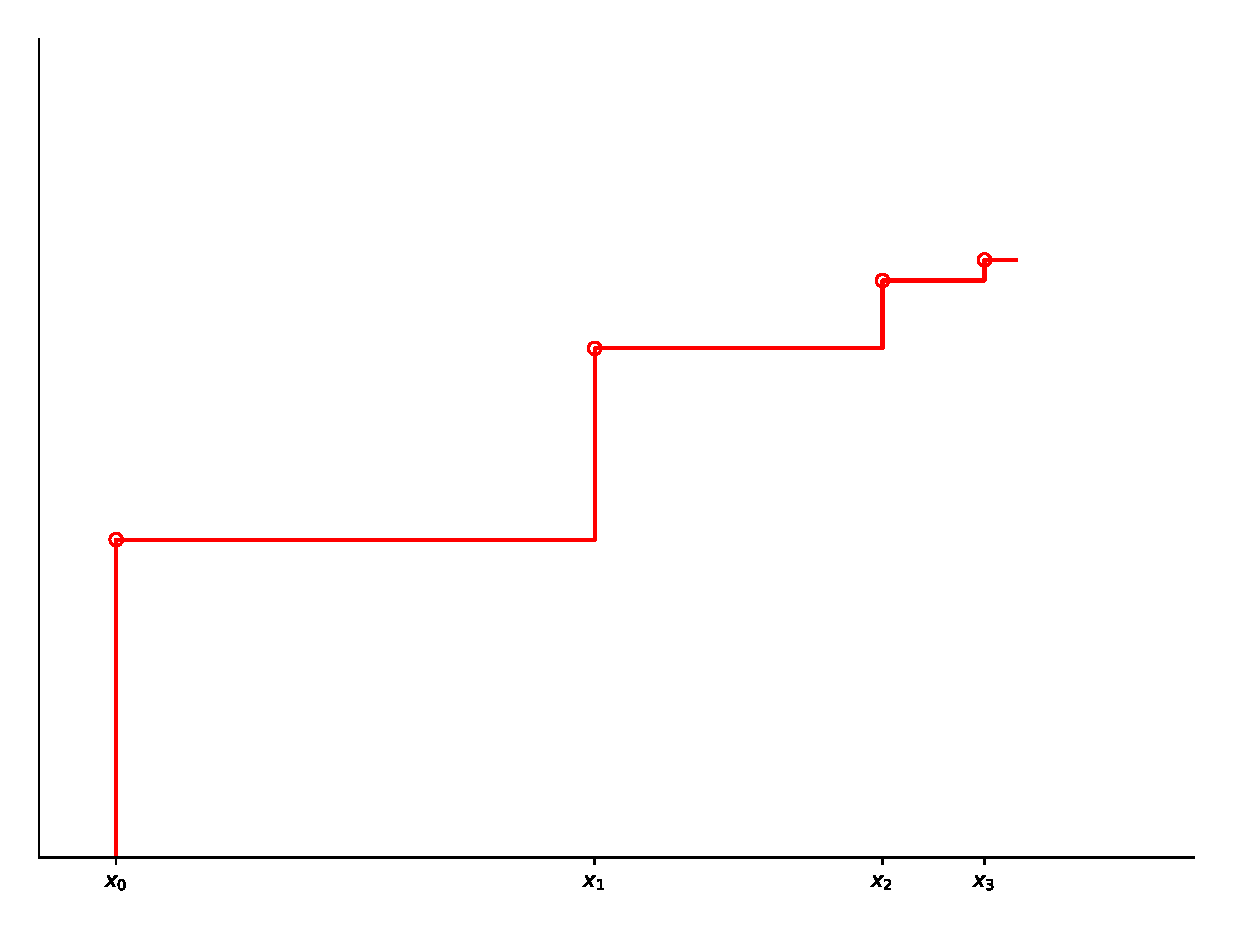
\includegraphics[width=0.4\textwidth]{direct_iteration_photo.eps}
    \end{figure}
  \end{frame}


  \begin{frame}[fragile]
    \frametitle{Direct Iteration Method}
    
    \textbf{Exercise 1: Find the root of}
    \[
    f(x) = x^3 -3x^2 - 3x - 4
    \]
    
    \textbf{Rewrite as:}
    \(
    x = (3x^2 + 3x + 4)^{(1/3)}
    \)
    \begin{itemize}
      \item Solve in Excel
      \item Solve in Python
    \end{itemize}
  
    \textbf{Rewrite as:}
    \(
    x = (x^3 - 3x^2 - 4)/3
    \)
    \begin{itemize}
      \item Solve in Excel
      \item Solve in Python
    \end{itemize}
  \end{frame}
  
  \begin{frame}[fragile]
    \frametitle{Intermezzo: Functions Revisited}
  
    \begin{itemize}
      \item In Python, you can define your own functions to reuse certain functionalities. We now define the mathematical function in a new file f.pyf.py:
      \begin{lstlisting}[language=Python]
def f(x):
    return x**2 + math.exp(x)
      \end{lstlisting}
      \item The first line contains the function keyword
      \item \( y \) is defined as output, \( x \) is defined as input
      \item The computation can use \( x \) as a scalar as well as a vector
      \begin{itemize}
        \item If \( x \) is a vector, \( y \) is also a vector.
      \end{itemize}
    \end{itemize}
  \end{frame}
  
  %% THE FOLLOWING SLIDE ONLY APPLIES TO MATLAB
  % \begin{frame}[fragile]
  %   \frametitle{Anonymous Functions}
  
  %   \begin{itemize}
  %     \item If you do not want to create a file, you can create an anonymous function:
  %     \begin{lstlisting}[language=Matlab]
  %     g = @(x) (x.^2 + exp(x));
  %     \end{lstlisting}
  %     \begin{itemize}
  %       \item \( g \): the name of the function
  %       \item \( @ \): indicator of a function handle
  %       \item \( x \): the input argument
  %     \end{itemize}
  %     \begin{lstlisting}[language=Matlab]
  %     g(0:0.1:1)
  %     \end{lstlisting}
      
  %     \item A function handle points to a function, but it behaves as a variable. You can pass a function handle as an argument.
  %   \end{itemize}
  % \end{frame}
  
  \begin{frame}[fragile]
    \frametitle{Passing Functions in Python}
  
    \begin{itemize}
      \item To solve \( f(x) = x^2 - 4x + 2 = 0 \) numerically, we can write a function that returns the value of \( f \):
      \begin{lstlisting}[language=Python]
def MyFunc(x):  # Note: case sensitive!!
    return x**2 - 4*x + 2
      \end{lstlisting}
      
      \item The function can be assigned to a variable as an alias:
      \begin{lstlisting}[language=Python]
f = MyFunc
a = 4
b = f(a)
      \end{lstlisting}
    
      \item We can then call a solving routine (e.g., \texttt{fsolve} from SciPy):
      \begin{lstlisting}[language=Python]
from scipy.optimize import fsolve
ans = fsolve(MyFunc, 5)
ans = fsolve(lambda x: x**2 - 4*x + 2, 5)
      \end{lstlisting}
    \end{itemize}
    
  \end{frame}
  
  \begin{frame}[fragile]
    \frametitle{Passing Functions in Python}
  
    \begin{itemize}
      \item We can also make our own function, that takes another function as an argument:
      \begin{lstlisting}[language=Python]
import matplotlib.pyplot as plt
import numpy as np
def draw_my_function(func):
    # Draws a function in the range [0, 10] using 20 data points.
    # 'func' is a function that can be any actual function.
    x = np.linspace(0, 10, 20)
    y = [func(val) for val in x]
    plt.plot(x, y, "-o")
    plt.show()
      \end{lstlisting}
  
      \item Now we can call the function with another function, either a lambda function or a common function:
      \begin{lstlisting}[language=Python]
f = lambda x: x**2 - 4*x + 2
draw_my_function(f)
      \end{lstlisting}
    \end{itemize}
  \end{frame}
  
  
  \begin{frame}[fragile]
    \frametitle{Direct Iteration Method}
    
    \textbf{Exercise 1: Find the root of}
    \[
    f(x) = x^3 -3x^2 - 3x - 4
    \]
    
    \textbf{Rewrite as:}
    \(
    x = (3x^2 + 3x + 4)^{1/3}
    \)
    \begin{itemize}
      \item Solve in Excel
      \item Solve in Python
    \end{itemize}
  
    \textbf{Rewrite as:}
    \(
    x = (x^3 - 3x^2 - 4)/3
    \)
    \begin{itemize}
      \item Solve in Excel
      \item Solve in Python
    \end{itemize}
  \end{frame}

  \begin{frame}[fragile]
    \frametitle{Direct Iteration Method}
  
      \textbf{Exercise 1: Find the root of \(f(x) = x^3 -3x^2 - 3x - 4\) with the direct iteration method in Excel}
      \vspace{0.5cm}
      \begin{columns}
        \column{0.40\textwidth}
      First method:\newline
      \vspace{0.2cm}
        \(
        \begin{array}{c|c|c}
        \text{Iteration} & \text{Formula} & \text{Result} \\
        \hline
        1 & (3x^2 + 3x + 4)^{(1/3)} & 2 \\
        2 & & 3.115 \\
        3 & & 3.489 \\
        \vdots & & \vdots \\
        10 & & 3.990 \\
        \end{array}
        \)
        \newline
        \newline
        \vspace{0.2cm}
        Converges!
        
        \column{0.40\textwidth}
        Second method:\newline
        \vspace{0.2cm}
        \(
        \begin{array}{c|c|c}
        \text{Iteration} & \text{Formula} & \text{Result} \\
        \hline
        1 & x = (x^3 - 3x^2 - 4)/3 & -1 \\
        2 & & -2.375 \\
        3 & & -11.439 \\
        \vdots & & \vdots \\
        10 & & \text{\#NUM!} \\
        \end{array}
        \)
        \newline
        \newline
        \vspace{0.2cm}
        Diverges!
      \end{columns}
  \end{frame}
  
  \begin{frame}[fragile]
    \frametitle{Direct Iteration Method}
    \textbf{Exercise 1: Find the root of \(f(x) = x^3 - 3x^2 - 3x - 4 = 0\) with the direct iteration method in Python}
  
    With a simple script:
    \begin{lstlisting}[language=Python]
x = 2.5
print(f"i: {0}, x: {x:.6e}")
for i in range(1, 21):
    x = (3*x**2 + 3*x + 4)**(1/3)
    print(f"i: {i}, x: {x:.6e}")
    \end{lstlisting}
    \begin{block}{Lesson}Not very flexible/reusable \(\rightarrow\) use functions\end{block}
  \end{frame}
  
  
  \begin{frame}[fragile]
  \frametitle{Direct Iteration Method}

  \textbf{Exercise 1: Find the root of the equation}
    \(
    f(x) = x^3 - 3x^2 - 3x - 4 = 0
    \)
    using the direct iteration method in Python.
  \begin{itemize}
    \item First, define the functions.
  \end{itemize}
  \begin{lstlisting}[language=Python]
def MyFnc1(x):
    return (3*x**2 + 3*x + 4)**(1/3)
  \end{lstlisting}
  \begin{lstlisting}[language=Python]
def MyFnc2(x):
    return (x**3 - 3*x**2 - 4) / 3
  \end{lstlisting}
\end{frame}

\begin{frame}[fragile]
  \frametitle{Direct Iteration Method}

  \textbf{Exercise 1: Find the root of the equation}
    \(
    f(x) = x^3 - 3x^2 - 3x - 4 = 0
    \)
    using the direct iteration method in Python.
  \begin{itemize}
    \item Then, create a function to carry out the Direct Iteration algorithm.
  \end{itemize}
  \begin{lstlisting}[language=Python]
def DirectIterationMethod(g, x, eps):
    itmax = 100
    it = 0
    y = g(x)
    print(f"i: {0}, x: {x:.6e}")
    while (abs(y - x) > eps) and (it < itmax):
        it += 1
        x = y
        y = g(x)
        print(f"i: {it}, x: {x:.6e}")
  \end{lstlisting}
\end{frame}

\begin{frame}[fragile]
  \frametitle{Direct Iteration Method}
  \textbf{Exercise 1: Find the root of the equation
    \(
    f(x) = x^3 - 3x^2 - 3x - 4 = 0
    \)
    using the direct iteration method in Python.}

  \begin{itemize}
    \item Finally, call the Direct Iteration function with the appropriate parameters.
  \end{itemize}
  \begin{lstlisting}[language=Python]
DirectIterationMethod(MyFnc1, 2.5, 1e-3)
DirectIterationMethod(MyFnc2, 2.5, 1e-3)
  \end{lstlisting}
  \begin{block}{Thinking}Discuss why it converges with \texttt{MyFnc1} and diverges with \texttt{MyFnc2}\end{block}
\end{frame}


  \begin{frame}[fragile]
    \frametitle{Direct Iteration Method}
  
    \begin{itemize}
      \item Exercise 1: Find the root of the equation
        \[
        f(x) = x^3 -3x^2 - 3x - 4 = 0
        \]
        using the direct iteration method.
      \item Observe that the method only works effectively when \(g'(x_i) < 1\). Even then, it may not converge quickly. 
    \end{itemize}
    \begin{columns}
      \column{0.5\textwidth}
    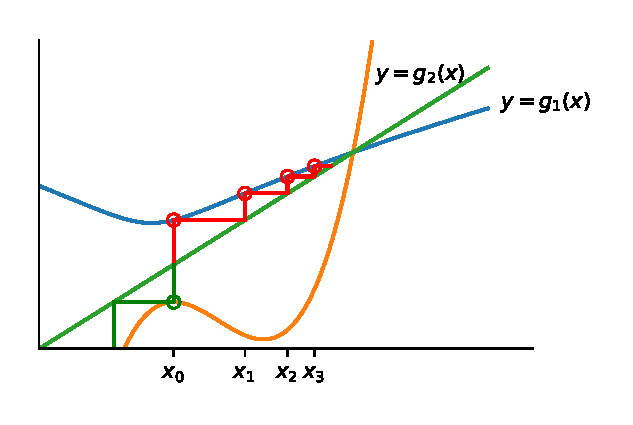
\includegraphics[width=0.95\textwidth]{direct_iteration_photo2.eps}
    \column{0.5\textwidth}
    \vspace{-0.5cm} 
    \begin{block}{Point}
      The iterations can be represented using the following relations:
      \begin{align*}
        & x_{i+1} = g(x_i) + g'(x_i)(x - x_i) \\
        & x_{i+2} = g(x_{i+1}) + g'(x_{i+1})(x_{i+1} - x_i) \\
        & \lvert x_{i+2} - x_{i+1} \rvert = \lvert g^\prime (x_i) \rvert \lvert x_{i+1} - x_i \rvert \\
        & \text{Convergence if } \lvert g^\prime (x_i) \rvert \leq 1
      \end{align*} 
    \end{block}    
    \end{columns}
  \end{frame}
  
  \begin{frame}[fragile]
    \frametitle{Bracketing}
    
    \textbf{Bracketing a root involves identifying an interval \((a, b)\) within which the function changes its sign.}
    \begin{columns}
    \column{0.4\textwidth}
      \vspace{0.25cm}
      

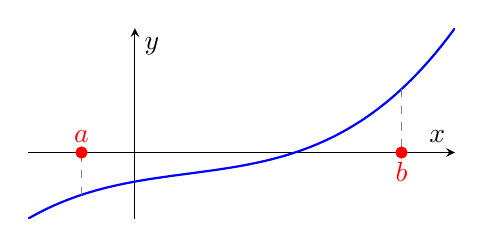
\begin{tikzpicture}
    \begin{axis}[
        axis lines = middle,
        xlabel = $x$,
        ylabel = {$y$},
        xtick = \empty,
        ytick = \empty,
        width=7cm,
        height=4cm
    ]
    
    \addplot[domain=-1:3, samples=100, color=blue, thick]{0.5*(x-.5)^3 + x-2}; % Change this function as per your requirement
    \addplot[mark=*,color=red] coordinates {(-0.5,0)} node[above] {$a$};
    \addplot[mark=*,color=red] coordinates {(2.5,0)}  node[below] {$b$};
    
    \draw [dashed, color=gray] (axis cs: -0.5,-3) -- (axis cs: -0.5,0);
    \draw [dashed, color=gray] (axis cs: 2.5,4.5) -- (axis cs: 2.5,0);
    
    \end{axis}
\end{tikzpicture}
     
      \vspace{0.25cm}
      
\begin{tikzpicture}
    \begin{axis}[
        axis lines = middle,
        axis on top,
        clip = false,
        xlabel = $x$,
        ylabel = {$y$},
        xtick = \empty,
        ytick = \empty,
        width=7cm,
        height=4cm
    ]
    
    
    \addplot[domain=-0.08:0.5, samples=100, color=tuesteel, thick]{-(x-0.5)^4 + 3}; % Change this function as per your requirement
    
    % Defining the main coordinates
    \coordinate (A) at (axis cs:0.05,2.95899);
    \coordinate (K) at (axis cs:0.1,2.9744);
    \coordinate (B) at (axis cs:0.3, 2.9984);
    \coordinate (Ax) at (axis cs:0.05,2.887);
    \coordinate (Kx) at (axis cs:0.1,2.887);
    \coordinate (Bx) at (axis cs:0.3,2.887);
    \coordinate (Ay) at (axis cs:0,2.95899);
    \coordinate (By) at (axis cs:0, 2.9984);
    \coordinate (Ky) at (axis cs:0,2.9744);
    
    \draw[red] (A) circle [radius=1.5pt];
    \draw[red] (B) circle [radius=1.5pt];
    \draw[red] (K) circle [radius=1.5pt];
    
    \draw[red, solid] (A) -- (Ax)   node[at end, below] {$a$};
    \draw[red, solid] (B) -- (Bx)   node[at end, below] {$b$};
    \draw[tuesteel, dashed] (K) -- (Kx) node[at end, below] {$k$};
    
    \draw[red, solid] (A) -- (Ay) node[at end, left] {$f(a)$};
    \draw[red, solid] (B) -- (By) node[at end, left] {$f(b)$};
    \draw[tuesteel, dashed] (K) -- (Ky) node[at end, left] {$f(k)$};
    
    \draw[red] (Ax) circle [radius=1.5pt];
    \draw[red] (Bx) circle [radius=1.5pt];
    \draw[tuesteel] (Kx) circle [radius=1.5pt];
    
    \end{axis}
    \end{tikzpicture}
      
    \column{0.5\textwidth}
    \begin{itemize}
      \item If \(f(a)\) and \(f(b)\) have opposite signs, it indicates that at least one root lies in the interval \((a, b)\), assuming the function is continuous in the interval.
      \item This is supported by the Intermediate Value Theorem.
    \end{itemize}
    \begin{block}{Intermediate value theorem}
      States that if \(f(x)\) is continuous on \([a, b]\) and \(k\) is a constant lying between \(f(a)\) and \(f(b)\), then there exists a value \(x \in [a, b]\) such that \(f(x) = k\).
    \end{block}
    \end{columns}
  
  \end{frame}

  \begin{frame}[fragile]
    \frametitle{Bracketing}

    \begin{block}{Point}
      Bracketing a root = Understanding that the function changes its sign in a specified interval, which is termed as bracketing a root.
    \end{block}

    \begin{columns}
    \column{0.4\textwidth}
    \vspace{0.25cm}
    

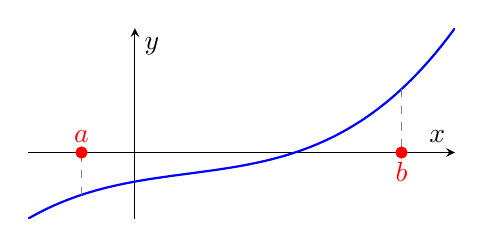
\begin{tikzpicture}
    \begin{axis}[
        axis lines = middle,
        xlabel = $x$,
        ylabel = {$y$},
        xtick = \empty,
        ytick = \empty,
        width=7cm,
        height=4cm
    ]
    
    \addplot[domain=-1:3, samples=100, color=blue, thick]{0.5*(x-.5)^3 + x-2}; % Change this function as per your requirement
    \addplot[mark=*,color=red] coordinates {(-0.5,0)} node[above] {$a$};
    \addplot[mark=*,color=red] coordinates {(2.5,0)}  node[below] {$b$};
    
    \draw [dashed, color=gray] (axis cs: -0.5,-3) -- (axis cs: -0.5,0);
    \draw [dashed, color=gray] (axis cs: 2.5,4.5) -- (axis cs: 2.5,0);
    
    \end{axis}
\end{tikzpicture}
     
    
    \column{0.5\textwidth}
    \textbf{General best advice}:
        \begin{itemize}
          \item Always bracket a root before attempting to converge on a solution.
          \item Never allow your iteration method to get outside the best bracketing bounds...
        \end{itemize}
    \end{columns}
  \end{frame}
  
  \begin{frame}[fragile]
    \frametitle{General Idea}
    
    \textbf{Potential issues to be cautious of while bracketing:}
    \begin{columns}
      \column{0.45\textwidth}
      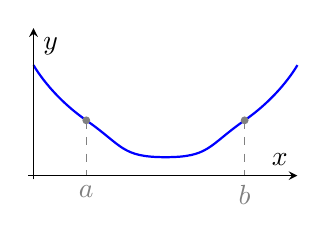
\begin{tikzpicture}
    \begin{axis}[
        axis lines = middle,
        axis on top,
        clip = false,
        xlabel = $x$,
        ylabel = {$y$},
        xtick = \empty,
        ytick = \empty,
        xmin=-0.1,xmax=5,
        ymin=-0.1,ymax=4,
        width=5cm,
        height=3.5cm
    ]
    
       % Define points
    \coordinate (A) at (0,3);
    \coordinate (B) at (1,1.5);
    \coordinate (C) at (2.5,0.5);
    \coordinate (D) at (4,1.5);
    \coordinate (E) at (5,3);

    \coordinate (Ax) at (0,0);
    \coordinate (Bx) at (1,0.0);
    \coordinate (Cx) at (2.5,0.0);
    \coordinate (Dx) at (4,0.0);
    \coordinate (Ex) at (5,0);

    % Draw smooth curve through the points
    \draw [blue, thick] plot[smooth, tension=1] coordinates {(A) (B) (C) (D) (E)};
    
    % Draw points for reference
    \draw[gray, dashed] (B) node[circle, fill=gray, inner sep=1pt] {} -- (Bx)   node[at end, below] {$a$};
    \draw[gray, dashed] (D) node[circle, fill=gray, inner sep=1pt] {} -- (Dx)   node[at end, below] {$b$};
    
    \end{axis}
    \end{tikzpicture}
\vspace{0.01cm}
      \newline 
      No answer (no root found)
      \vspace{0.8cm}
      
      \input{tikzplots/one_solution.tex}\vspace{0.01cm}
      \newline 
      Ideal scenario with one root found
      \vspace{0.8cm}
      
      \column{0.45\textwidth}
      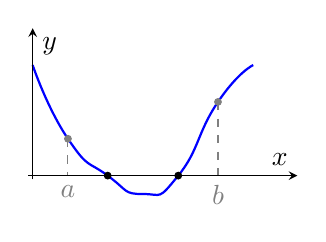
\begin{tikzpicture}
    \begin{axis}[
        axis lines = middle,
        axis on top,
        clip = false,
        xlabel = $x$,
        ylabel = {$y$},
        xtick = \empty,
        ytick = \empty,
        xmin=-0.1,xmax=6,
        ymin=-0.1,ymax=4,
        width=5cm,
        height=3.5cm
    ]
    
       % Define points0. , 0.8, 1.7, 2.5, 3.3, 4.2, 5. ]
    \coordinate (A) at (+0.0, +3.0);
    \coordinate (B) at (+0.8, +1.0);
    \coordinate (C) at (+1.7, +0.0);
    \coordinate (D) at (+2.5, -0.5);
    \coordinate (E) at (+3.3, +0.0);
    \coordinate (F) at (+4.2, +2.0);
    \coordinate (G) at (+5.0, +3.0);

    \coordinate (Ax) at (+0.0, +0.0);
    \coordinate (Bx) at (+0.8, +0.0);
    \coordinate (Cx) at (+1.7, +0.0);
    \coordinate (Dx) at (+2.5, -0.0);
    \coordinate (Ex) at (+3.3, +0.0);
    \coordinate (Fx) at (+4.2, +0.0);
    \coordinate (Gx) at (+5.0, +0.0);
    
    % Draw smooth curve through the points
    \draw [blue, thick] plot[smooth, tension=1] coordinates {(A) (B) (C) (D) (E) (F) (G)};
    
    % Draw points for reference
    \draw[gray, dashed] (B) node[circle, fill=gray, inner sep=1pt] {} -- (Bx)   node[at end, below] {$a$};
    \draw[gray, dashed] (F) node[circle, fill=gray, inner sep=1pt] {} -- (Fx)   node[at end, below] {$b$};

    \draw (C) node[circle, fill=black, inner sep=1pt] {};
    \draw (E) node[circle, fill=black, inner sep=1pt] {};
    
    
    
    
    \end{axis}
    \end{tikzpicture}
\vspace{0.01cm}
      \newline 
      Oops! Encountering two roots
      \vspace{0.8cm}
      
      \input{tikzplots/three_solutions.tex}\vspace{0.01cm}
      \newline 
      Finding three roots (might work temporarily)
      \vspace{0.8cm}
    \end{columns}
  
    % Add any visual or diagram here, replace 'path/to/your/diagram' with the actual path to your diagram file
    % \includegraphics[width=0.5\textwidth]{path/to/your/diagram}
  \end{frame}

  \begin{frame}[fragile]
    \frametitle{Bracketing}
  
    \textbf{Exercise 2:}
    \begin{itemize}
      \item Write a Python function to bracket a function, starting with an initially guessed range \(x_1\) and \(x_2\) through the expansion of the interval.
      \item Develop a program to ascertain the minimum number of roots existing within the \(x_1\) and \(x_2\) interval.
      \item Note: These functions can be integrated to formulate a function that yields bracketing intervals for diverse roots.
    \end{itemize}
  \end{frame}
  
  \begin{frame}[fragile]
    \frametitle{Bracketing}
  
    \textbf{Exercise 2: Function to Bracket a Function}
    
    \begin{itemize}
      \item Initially, if feasible, draft a graph using the following Python commands:
        \begin{lstlisting}[language=Python]
import matplotlib.pyplot as plt
import numpy as np

x = np.linspace(0, 5, 50)
y = x**2 - 4*x + 2
plt.figure()
plt.plot(x, y, x, np.zeros(len(x)))
plt.axis('tight')
plt.grid(True)
plt.show()
        \end{lstlisting}
      \item This graphical representation instantly reveals the existence of two roots, evaluated as:
        \[
        x_1 = 2 - \sqrt{2} \approx 0.59
        \]
        \[
        x_2 = 2 + \sqrt{2} \approx 3.41
        \]
    \end{itemize}
  
    % Add your graph here, replace 'path/to/your/graph' with the actual path to your graph file
    % \includegraphics[width=0.5\textwidth]{path/to/your/graph}
  \end{frame}
  
  \begin{frame}[fragile]
    \frametitle{Bracketing}
  
    \textbf{Exercise 2: Function to Bracket a Function}
    \begin{itemize}
      \item Devise a Python function to bracket a function with an initial guessed range of \( x_1 \) and \( x_2 \) through the expansion of the interval.
      \item Create a program to determine the minimum number of roots within the \( x_1 \) and \( x_2 \) interval.
      \item \textbf{Remark}: These functions can be synergized to build a function that designates bracketing intervals for varying roots.
    \end{itemize}
  \end{frame}
  
  \begin{frame}[fragile]
    \frametitle{Bracketing}
    
    \textbf{Exercise 2: Function to Bracket a Function}
    \begin{columns}
      \column{0.5\textwidth}
      \begin{lstlisting}[language=Python,basicstyle=\tiny]
def find_root_by_bracketing(func, x1, x2, tol=1e-6, max_iter=1000):
  # Ensure the bracket is valid
  if func(x1) * func(x2) > 0:
      print('The bracket is invalid. The function must have opposite signs at the two endpoints.')
      return False

  # Loop until we find the root or exceed the maximum number of iterations
  for i in range(max_iter):
      # Find the midpoint
      x_mid = (x1 + x2) / 2
      
      # Check if we found the root
      if abs(func(x_mid)) < tol:
          print(f'Root found: {x_mid}')
          return True
      
      # Narrow down the bracket
      if func(x_mid) * func(x1) < 0:
          x2 = x_mid
      else:
          x1 = x_mid

  # If we reach here, we did not find the root within the maximum number of iterations
  print('Failed to find the root within the maximum number of iterations.')
  return False
      \end{lstlisting}
      \column{0.5\textwidth}
      \textbf{Steps:}
      \begin{itemize}
        \item Formulate a function to augment the interval \((x_1, x_2)\) up to a maximum of 250 iterations or until a root is discovered.
        \item The function should:
          \begin{itemize}
            \item Return true if a root is found, and false otherwise.
            \item Showcase the results.
          \end{itemize}
      \end{itemize}
    \end{columns}
  \end{frame}

  \begin{frame}[fragile]
    \frametitle{Bracketing}
    
    \textbf{Exercise 2: Function to Bracket a Function}
    \begin{columns}
    \column{0.49\textwidth}
    \begin{lstlisting}[language=Python,basicstyle=\scriptsize]
def brak(func, x1, x2, n):
    nroot = 0
    dx = (x2 - x1) / n
    xb1 = []
    xb2 = []

    x = x1
    for i in range(n):
        x += dx
        if func(x) * func(x - dx) <= 0:
            nroot += 1
            xb1.append(x - dx)
            xb2.append(x)

    for i in range(nroot):
        print(f'Root {i+1} in bracketing interval [{xb1[i]}, {xb2[i]}]')
    else:
        if nroot == 0:
            print('No roots found!')
    \end{lstlisting}
    \column{0.49\textwidth}
    \textbf{Steps:}
    \begin{itemize}
      \item The function subdivides the interval \((x_1, x_2)\) into \(n\) parts to check for at least one root.
      \item It returns the left and right boundaries of the intervals where roots are found in arrays xb1 and xb2.
    \end{itemize}
  \end{columns}
  \end{frame}
  
  \begin{frame}[fragile]
    \frametitle{Bisection Method}
  
    Bisection Algorithm:
    \begin{itemize}
      \item Within a certain interval, the function crosses zero, indicated by a change in sign.
      \item Evaluate the function value at the midpoint of the interval and examine its sign.
      \item The midpoint then supersedes the limit sharing its sign.
    \end{itemize}
  
    \begin{columns}
    \column{0.45\textwidth}
    \vspace{0.5cm}
    \centering
    \begin{tikzpicture}
    \begin{axis}[
            axis lines = middle,
            xlabel = $x$,
            ylabel = {$y$},
            xtick = \empty,
            ytick = \empty,
            width=\textwidth,
            ymin=-2.1
        ]
    
        % USED BISECTION.py and CHATGPT TO GET THE COORDINATES
        \coordinate (Iter0) at (-1.5, -0.39);
        \coordinate (Iter1) at (4, 2.16);
        \coordinate (Iter2) at (-0.66, -0.85);
        \coordinate (Iter3) at (0.65, 0.69);
        \coordinate (Iter4) at (0.06, -0.2);
        \coordinate (Iter5) at (0.19, 0.01);

        
        \coordinate (Iter0x) at (-1.5, 0.0);
        \coordinate (Iter1x) at (4, 0.0);
        \coordinate (Iter2x) at (-0.66, 0.0);
        \coordinate (Iter3x) at (0.65,0.0);
        \coordinate (Iter4x) at (0.06,0.0);
        \coordinate (Iter5x) at (0.19,0.0);

        
        \addplot[domain=-2:4.5, samples=100, color=blue, thick]{sin(deg(x*2-0.5))*.6+2/5*x}; % Change this function as per your requirement
        \draw[gray, dashed] (Iter0) -- (Iter0x)   node[black, at start, above] {};
        \draw[gray, dashed] (Iter1) -- (Iter1x)   node[black, at start, above] {};
        \draw (Iter0x) node[blue, above] {$a$};
        \draw (Iter1x) node[blue, below] {$b$};
        \draw[gray, dashed] (Iter2) -- (Iter2x)   node[black, at start, below] {$1$};
        \draw[gray, dashed] (Iter3) -- (Iter3x)   node[black, at start, below] {$2$};
        \draw[gray, dashed] (Iter4) -- (Iter4x)   node[black, at start, below] {$3$};
        \draw[gray, dashed] (Iter5) -- (Iter5x)   node[black, at start, above] {$4$};
    
        \fill[cyan] (Iter0) circle (1pt);
        \fill[cyan] (Iter1) circle (1pt);
        \fill[cyan] (Iter2) circle (1pt);
        \fill[cyan] (Iter3) circle (1pt);
        \fill[cyan] (Iter4) circle (1pt);
        \draw[blue, solid] (Iter0) circle (1pt);
        \draw[blue, solid] (Iter1) circle (1pt);
        \draw[blue, solid] (Iter2) circle (1pt);
        \draw[blue, solid] (Iter3) circle (1pt);
        \draw[blue, solid] (Iter4) circle (1pt);
        \draw[gray, dash pattern={on 0.5pt off 0.2pt}] (Iter5) circle (2pt);
        
        
    \end{axis}
    \end{tikzpicture}
    \column{0.45\textwidth}
  
    \begin{block}{Properties}
    \begin{itemize}
      \item Pros: The method is infallible.
      \item Cons: Convergence is relatively slow.
    \end{itemize}
  \end{block}
  \end{columns}
  \end{frame}
  

  \begin{frame}[fragile]
    \frametitle{Bisection Method}
  
    \textbf{Exercise 3}
    \begin{itemize}
      \item Write a function in Excel to find a root of a function using the bisection method.
      \item Assume that an initial bracketing interval \((x_1, x_2)\) is provided.
      \item Specify the required tolerance.
      \item Output the required number of iterations.
      \item Implement the same in Python.
    \end{itemize}
  \end{frame}
  
  \begin{frame}[fragile]
    \frametitle{Exercise 3}
    
    \textbf{Bisection Method in Excel:}
    \begin{table}[]
      \begin{tabular}{|c|c|c|c|c|c|c|c|}
      \hline
      it & \(x_1\) & \(x_2\) & \(f_1\) & \(f_2\) & xmid & fmid & Interval Size \\
      \hline
      0 & -2 & 2 & 14 & -2 & 0 & 2 & 4 \\
      1 & 0 & 2 & 2 & -2 & 1 & -1 & 2 \\
      \vdots & \vdots & \vdots & \vdots & \vdots & \vdots & \vdots & \vdots \\
      25 & 0.585786 & 0.585786 & \(1 \times 10^{-7}\) & \(-6.8 \times 10^{-8}\) & 0.585786 & \(1.58 \times 10^{-8}\) & \(5.96 \times 10^{-8}\) \\
      \hline
      \end{tabular}
    \end{table}
    
    Note: The table represents a sequence of iterations showing how the bisection method converges to a root with each step, demonstrating variable updates and interval size reduction. 
  
  \end{frame}
  
  \begin{frame}[fragile]
    \frametitle{Bisection Method}
  
    \textbf{Exercise 3: Python Implementation}
    \begin{columns}
      \column{0.45\textwidth}
      \begin{lstlisting}[language=Python,basicstyle=\tiny]
def bisection(func, a, b, tol, maxIter):
    if func(a) * func(b) > 0:
        print('Error: f(a) and f(b) must have different signs.')
        return None

    iter = 0
    while (b - a) / 2 > tol:
        iter += 1
        if iter >= maxIter:
            print('Maximum iterations reached')
            return None

        c = (a + b) / 2
        print(f'Iteration {iter}: Current estimate: {c}')

        if func(c) == 0:
            return c

        if np.sign(func(c)) != np.sign(func(a)):
            b = c
        else:
            a = c

    return (a + b) / 2
      \end{lstlisting}
  
      \column{0.45\textwidth}
      \vspace{-1cm}
      \begin{itemize}
      \item Criterion used for both the function value and the step size.
      \item While loop usually requires protection for a maximum number of iterations.
      \item Bisection is sure to converge.
      \item Root found in 25 iterations. Can we optimize it further?
    \end{itemize}
  \end{columns}
  \end{frame}
  
  
  \begin{frame}[fragile]
    \frametitle{Bisection Method}
    
    \textbf{Required Number of Iterations:}
    \begin{itemize}
      \item Interval bounds containing the root decrease by a factor of 2 after each iteration.
      \begin{columns}
        \column{0.40\textwidth}
      \[
      \varepsilon_{n+1} = \frac{1}{2}\varepsilon_n \quad\Rightarrow\quad \boxed{n = \log _2\frac{\varepsilon_0}{tol}}
      \]
      \column{0.55\textwidth}
      \begin{align*}
        \varepsilon_0 &= \text{initial bracketing interval}, \\
        tol &= \text{desired tolerance}.
        \end{align*}
      \end{columns}
      \item After \(50\) iterations, the interval is decreased by a factor of \(2^{50} = 10^{15}\).
      \item Consider machine accuracy when setting tolerance.
      \item Order of convergence is \(1\):
      \begin{columns}
        \column{0.30\textwidth}
      \[
      \boxed{\varepsilon_{n+1} = K\varepsilon_n ^ m}
      \]
      \column{0.69\textwidth}
      \begin{itemize}
        \item \(m = 1\): linear convergence.
        \item \(m = 2\): quadratic convergence.
      \end{itemize}
      \end{columns}
      \vspace{0.25cm}
      \item Bisection method will:
      \begin{itemize}
        \item Find one of the roots if there is more than one.
        \item Find the singularity if there is no root but a singularity exists.
      \end{itemize}
    \end{itemize}
  \end{frame}


  \begin{frame}[fragile]
    \frametitle{Secant and False Position Method}
  
    \textbf{Secant/False Position (Regula Falsi) Method}
      \begin{itemize}
        \item Provides faster convergence given sufficiently smooth behavior.
        \item Differs from the bisection method in the choice of the next point:
        \begin{itemize}
          \item \textbf{Bisection}: selects the mid-point of the interval.
          \item \textbf{Secant/False position}: chooses the point where the approximating line intersects the axis.
        \end{itemize}
        \item Adopts a new estimate by discarding one of the boundary points:
        \begin{itemize}
          \item \textbf{Secant}: retains the most recent of the previous estimates.
          \item \textbf{False position}: maintains the prior estimate with the opposite sign to ensure the points continue to bracket the root.
        \end{itemize}
      \end{itemize}
  \end{frame}
  
  \begin{frame}[fragile]
    \frametitle{Secant and False Position Method: Comparison}

    \begin{columns}
      \column{0.49\textwidth}
        \textbf{Secant Method}
        \vspace{0.1cm}
        \newline 
        
        \begin{tikzpicture}
    \begin{axis}[
            axis lines = middle,
            xlabel = $x$,
            ylabel = {$y$},
            xtick = \empty,
            ytick = \empty,
            width=\textwidth,
            ymin=-2.1
        ]
    
        % USED BISECTION.py and CHATGPT TO GET THE COORDINATES
        \coordinate (Iter0) at (-1.5, -0.39);
        \coordinate (Iter1) at (4, 2.16);
        \coordinate (Iter2) at (-0.66, -0.85);
        \coordinate (Iter3) at (0.65, 0.69);
        \coordinate (Iter4) at (0.06, -0.2);
        \coordinate (Iter5) at (0.19, 0.01);

        
        \coordinate (Iter0x) at (-1.5, 0.0);
        \coordinate (Iter1x) at (4, 0.0);
        \coordinate (Iter2x) at (-0.66, 0.0);
        \coordinate (Iter3x) at (0.65,0.0);
        \coordinate (Iter4x) at (0.06,0.0);
        \coordinate (Iter5x) at (0.19,0.0);

        
        \addplot[domain=-2:4.5, samples=100, color=blue, thick]{sin(deg(x*2-0.5))*.6+2/5*x}; % Change this function as per your requirement
        \draw[gray, dashed] (Iter0) -- (Iter0x)   node[black, at start, above] {};
        \draw[gray, dashed] (Iter1) -- (Iter1x)   node[black, at start, above] {};
        \draw (Iter0x) node[blue, above] {$a$};
        \draw (Iter1x) node[blue, below] {$b$};
        \draw[gray, dashed] (Iter2) -- (Iter2x)   node[black, at start, below] {$1$};
        \draw[gray, dashed] (Iter3) -- (Iter3x)   node[black, at start, below] {$2$};
        \draw[gray, dashed] (Iter4) -- (Iter4x)   node[black, at start, below] {$3$};
        \draw[gray, dashed] (Iter5) -- (Iter5x)   node[black, at start, above] {$4$};
    
        \fill[cyan] (Iter0) circle (1pt);
        \fill[cyan] (Iter1) circle (1pt);
        \fill[cyan] (Iter2) circle (1pt);
        \fill[cyan] (Iter3) circle (1pt);
        \fill[cyan] (Iter4) circle (1pt);
        \draw[blue, solid] (Iter0) circle (1pt);
        \draw[blue, solid] (Iter1) circle (1pt);
        \draw[blue, solid] (Iter2) circle (1pt);
        \draw[blue, solid] (Iter3) circle (1pt);
        \draw[blue, solid] (Iter4) circle (1pt);
        \draw[gray, dash pattern={on 0.5pt off 0.2pt}] (Iter5) circle (2pt);
        
        
    \end{axis}
    \end{tikzpicture}
      
        \begin{itemize}
          \item Slightly faster convergence:
          \[
          \lim_{n \to \infty} \vline\varepsilon_{n+1}\vline = K\vline\varepsilon_n\vline^{1.618}
          \]
        \end{itemize}
  
      \column{0.49\textwidth}
        \textbf{False Position Method}
        \vspace{0.3cm}
        \newline 
        % \begin{tikzpicture}
          \begin{tikzpicture}[font=\footnotesize]
    \begin{axis}[
            axis lines = middle,
            xlabel = $x$,
            ylabel = {$y$},
            xtick = \empty,
            ytick = \empty,
            ymin=-2.1,
            width=\textwidth
        ]
    
        \coordinate (Iter0) at (-1.5, -0.39);
        \coordinate (Iter1) at (4, 2.16);
        \coordinate (Iter2) at (-0.66, -0.85);
        \coordinate (Iter3) at (0.65, 0.69);
        \coordinate (Iter4) at (0.06, -0.2);
        \coordinate (Iter5) at (0.19, 0.01);

        \coordinate (Iter0x) at (-1.5,  0.0);
        \coordinate (Iter1x) at (4,  0.0);
        \coordinate (Iter2x) at (-0.66, 0.0);
        \coordinate (Iter3x) at (0.65,  0.0);
        \coordinate (Iter4x) at (0.06,  0.0);
        \coordinate (Iter5x) at (0.19, 0.0);

        \addplot[domain=-2:4.5, samples=100, color=tuesteel, thick]{sin(deg(x*2-0.5))*.6+2/5*x}; % Change this function as per your requirement
        \draw[tuesteel, dashed] (Iter0) -- (Iter0x)   node[black, at start, above] {};
        \draw[tuesteel, dashed] (Iter1) -- (Iter1x)   node[black, at start, above] {};
        \draw (Iter0x) node[tuesteel, above] {$a$};
        \draw (Iter1x) node[tuesteel, below] {$b$};
        \draw[tuesteel, dashed] (Iter2) -- (Iter2x)   node[black, at start, below] {$2$};
        \draw[tuesteel, dashed] (Iter3) -- (Iter3x)   node[black, at start, below] {$3$};
        \draw[tuesteel, dashed] (Iter4) -- (Iter4x)   node[black, at start, below] {$4$};
        \draw[tuesteel, dashed] (Iter5) -- (Iter5x)   node[black, at start, below] {$5$};
    
        \fill[cyan] (Iter0) circle (1pt);
        \fill[cyan] (Iter1) circle (1pt);
        \fill[cyan] (Iter2) circle (1pt);
        \fill[cyan] (Iter3) circle (1pt);
        \fill[cyan] (Iter4) circle (1pt);
        \draw[tuesteel, solid] (Iter0) circle (1pt);
        \draw[tuesteel, solid] (Iter1) circle (1pt);
        \draw[tuesteel, solid] (Iter2) circle (1pt);
        \draw[tuesteel, solid] (Iter3) circle (1pt);
        \draw[tuesteel, solid] (Iter4) circle (1pt);
        \draw[tuesteel, dash pattern={on 0.5pt off 0.2pt}] (Iter5) circle (2pt);
        
        
    \end{axis}
    \end{tikzpicture}
        % \end{tikzpicture}
        \begin{itemize}
          \item Guaranteed convergence
        \end{itemize}
    \end{columns}
  \end{frame}

\begin{frame}[fragile]
  \frametitle{Secant and False Position Method}

  \textbf{Exercise 4:}
  \begin{itemize}
    \item Write a function in Excel and Python to find a root of a function using the Secant and False position methods.
    \item Assume that an initial bracketing interval \((x_1, x_2)\) is provided.
    \item Specify the required tolerance.
    \item Output the required number of iterations.
    \item Compare the bisection, false position, and secant methods.
  \end{itemize}
\end{frame}

\begin{frame}[fragile]
  \frametitle{Secant and False Position Method}

  \textbf{Exercise 4:}
  \begin{itemize}
    \item Determination of the abscissa of the approximating line:
    \begin{columns}
    \column{0.5\textwidth}
    \begin{itemize}
      \item Determine the approximating line using the expression:
      \[
      f(x) \approx f(a) + \frac{f(b) - f(a)}{b - a}(x - a)
      \]
      \item Determine the abscissa where \(f(x^*) = 0\):
        \begin{align*}
          x^* &= a - \frac{f(a)(b - a)}{f(b) - f(a)}\\
              &= \frac{af(b) - bf(a)}{f(b) - f(a)}
        \end{align*}
      \end{itemize}
        \column{0.5\textwidth}
        \vspace{0.5cm}
        \begin{tikzpicture}
    \begin{axis}[
            axis lines = middle,
            xlabel = $x$,
            ylabel = {$y$},
            xtick = \empty,
            ytick = \empty,
            width=\textwidth,
            ymin=-1.1
        ]
    
        % USED BISECTION.py and CHATGPT TO GET THE COORDINATES
        \coordinate (Iter0) at (-1.5, -0.39);
        \coordinate (Iter1) at (4, 2.16);
        \coordinate (mid) at (-0.6606041118839534, 0.0);        
        
        \coordinate (Iter0x) at (-1.5, 0.0);
        \coordinate (Iter1x) at (4, 0.0);
        
        
        \addplot[domain=-2:4.5, samples=100, color=blue, thick]{sin(deg(x*2-0.5))*.6+2/5*x}; % Change this function as per your requirement
        \draw[gray, dashed, thin] (Iter0) -- (Iter0x)   node[black, at start, above] {};
        \draw[gray, dashed, thin] (Iter1) -- (Iter1x)   node[black, at start, above] {};
        \draw (Iter0x) node[blue, above] {$a$};
        \draw (Iter1x) node[blue, below] {$b$};
        \draw[gray, dashed] (Iter0) -- (Iter1);
        \draw (mid) node[black, above] {$x^*$};
        \fill[cyan] (mid) circle (1pt);
        \draw[blue, solid] (mid) circle (1pt);
        \fill[cyan] (Iter0) circle (1pt);
        \draw[blue, solid] (Iter0) circle (1pt);
        \fill[cyan] (Iter1) circle (1pt);
        \draw[blue, solid] (Iter1) circle (1pt);
        
        
        
    \end{axis}
    \end{tikzpicture}
      \end{columns}
  \end{itemize}
  Note: In the above equations, \(a\) and \(b\) are the initial guesses/boundaries where the root is suspected to be, and \(f(x)\) is the function for which we are finding the root.
\end{frame}


\begin{frame}[fragile]
    \frametitle{Secant and False Position Method}

    \textbf{Exercise 4:}
    \begin{itemize}
      \item Write a function in Excel and Python to find a root of a function using the Secant and the False position methods.
      \item Assume that an initial bracketing interval \((x_1, x_2)\) is provided.
      \item Specify the required tolerance.
      \item Output the required number of iterations.
      \item Compare the bisection, false position, and secant methods.
    \end{itemize}
\end{frame}

\begin{frame}[fragile]
    \frametitle{Secant and False Position Method}

    \textbf{Exercise 4: False Position Method in Excel}
    \begin{table}[]
      \begin{tabular}{|l|l|l|l|l|l|l|l|}
      \hline
      iteration & xa      & xb     & fa      & fb     & x absc  & fabsc   & interval \\ \hline
      0         & -1.5000 & 4.0000 & -0.3895 & 2.1628 & -0.6606 & -0.8455 & 5.5000   \\ \hline
      1         & -0.6606 & 4.0000 & -0.8455 & 2.1628 & 0.6493  & 0.6896  & 4.6606   \\ \hline
      2         & -0.6606 & 0.6493 & -0.8455 & 0.6896 & 0.0609  & -0.1972 & 1.3099   \\ \hline
      3         & 0.0609  & 0.6493 & -0.1972 & 0.6896 & 0.1917  & 0.0070  & 0.5884   \\ \hline
      4         & 0.0609  & 0.1917 & -0.1972 & 0.0070 & 0.1873  & -0.0001 & 0.1308   \\ \hline
      5         & 0.1873  & 0.1917 & -0.0001 & 0.0070 & 0.1874  & 0.0000  & 0.0045   \\ \hline
      6         & 0.1874  & 0.1917 & 0.0000  & 0.0070 & 0.1874  & 0.0000  & 0.0044   \\ \hline
      7         & 0.1874  & 0.1917 & 0.0000  & 0.0070 & 0.1874  & 0.0000  & 0.0044   \\ \hline
      \end{tabular}
      \end{table}
    Relevant expressions: 
    \begin{itemize}
      \item \texttt{a=IF((a*fa)<0,a,xbsc)}
      \item \texttt{b=IF((b*fb)<0,b,xbsc)}
      \item \texttt{xbsc=a - fa*(xb-xa)/(fb-fa)}
    \end{itemize}
\end{frame}

\begin{frame}[fragile]
    \frametitle{Secant and False Position Method}

    \textbf{Exercise 4:}
    \begin{itemize}
        \item Write a function in Excel and Python to find a root of a function using the Secant and the False position methods.
        \item Assume that an initial bracketing interval \((x_1, x_2)\) is provided.
        \item Also the required tolerance is specified.
        \item Also output the required number of iterations.
        \item Compare the bisection, false position, and secant methods.
    \end{itemize}
\end{frame}


\begin{frame}[fragile]
    \frametitle{Secant and False Position Method}

    \textbf{Exercise 4: Secant method in excel}
    
    \begin{table}[]
      \begin{tabular}{|l|l|l|}
      \hline
      iteration & x     & f     \\ \hline
      -1        & 2.0000  & 0.5895  \\ \hline
      0         & -1.0000 & -0.7591 \\ \hline
      1         & 0.6886  & 0.7368  \\ \hline
      2         & -0.1431 & -0.4819 \\ \hline
      3         & 0.1857  & -0.0026 \\ \hline
      4         & 0.1875  & 0.0002  \\ \hline
      5         & 0.1874  & 0.0000  \\ \hline
      \end{tabular}
      \end{table}
    \textbf{Relevant expressions:}
    \[
    x_{n} = x_{n-1} - f(x_{n-1})\frac{x_{n-1} - x_{n-2}}{f(x_{n-1}) - f(x_{n-2})}
    \]
    \[
    f_{n} = f(x_{n})
    \]
\end{frame}

\begin{frame}[fragile]
  \frametitle{Secant and False Position Method}

  \textbf{Exercise 4: False position method in Python}
  \begin{lstlisting}[language=Python,basicstyle=\scriptsize]
def false_position(f, x0, x1, tol, max_iter):
    if f(x0) * f(x1) > 0:
        raise ValueError('f(x0) and f(x1) must have different signs.')

    history = []

    for i in range(max_iter):
        x2 = x1 - f(x1) * (x1 - x0) / (f(x1) - f(x0))
        history.append(x2)

        if abs(f(x2)) < tol:
            break

        if f(x2) * f(x0) < 0:
            x1 = x2
        else:
            x0 = x2

    root = x2
    return root, history
  \end{lstlisting}
  
  Calling the function:
  \begin{lstlisting}[language=Python,basicstyle=\scriptsize]
secant_method(lambda x: x**2 - 4*x + 2, 0, 2, 1e-7, 100)
  \end{lstlisting}
\end{frame}

\begin{frame}[fragile]
  \frametitle{Secant and False Position Method}

  \textbf{Exercise 4: Secant method in Python}
  \begin{lstlisting}[language=Python, basicstyle=\scriptsize]
def secant_method(f, x0, x1, tol, max_iter):
    history = [x0, x1]
    
    for i in range(1, max_iter):
        x2 = x1 - f(x1) * (x1 - x0) / (f(x1) - f(x0))
        history.append(x2)

        if abs(x2 - x1) < tol:
            break

        x0 = x1
        x1 = x2

    root = x1
    return root, history
  \end{lstlisting}
  
  Calling the function:
  \begin{lstlisting}[language=Python, basicstyle=\small]
false_position(lambda x: x**2 - 4*x + 2, 0, 2, 1e-7, 100)
  \end{lstlisting}
\end{frame}

\begin{frame}[fragile]
  \frametitle{Comparison of Methods}

  \textbf{Exercise 4:}
  \begin{itemize}
    \item \( \text{tol}_{\text{eps}}, \text{tol}_{\text{func2}} = 1e-15, \quad \text{and} \quad (x_1, x_2) = (0,2) \)
    \item \( f(x) = x^2 - 4x + 2 = 0 \)
  \end{itemize}

  \begin{table}
      \begin{tabular}{|l|c|}
          \hline
          Method & Nr. of iterations \\
          \hline
          Bisection & 52 \\
          False position & 22 \\
          Secant & 9 \\
          \hline
      \end{tabular}
  \end{table}

  \begin{lstlisting}[language=Python, basicstyle=\small]
from scipy.optimize import root_scalar

root_scalar(lambda x: x**2 - 4*x + 2, method='brentq', bracket=[0, 2], xtol=1e-15)
  \end{lstlisting}
  
  Note the initial bracketing steps in root\_scalar!
\end{frame}


\begin{frame}[fragile]
    \frametitle{Brent's Method}

    \textbf{Features of Brent's method:}
    \begin{itemize}
        \item Superlinear convergence with the sureness of bisection
        \item Keeps track of superlinear convergence, and if not achieved, alternates with bisection steps, ensuring at least linear convergence
        \item Implemented in MATLAB's \texttt{scipy.optimize.fzero} function:
        \begin{itemize}
            \item Utilizes root-bracketing
            \item Bisection/secant/inverse quadratic interpolation
        \end{itemize}
        \item Inverse quadratic interpolation:
        \begin{itemize}
            \item Uses three prior points to fit an inverse quadratic function ($x(y)$)
            \item Involves contingency plans for roots falling outside the brackets
        \end{itemize}
    \end{itemize}

\end{frame}

\begin{frame}[fragile]
  \frametitle{Brent's method}
  \textbf{Formulas:}
  \begin{align*}
    x &= b + \frac{P}{Q}, & R &= \frac{f(b)}{f(c)} \\
    P &= S\left[T(R-T)(c-b) - (1-R)(b-a)\right], & S &= \frac{f(b)}{f(a)} \\
    Q &= (T-1)(R-1)(S-1), & T &= \frac{f(a)}{f(c)}
    \end{align*}
    \begin{itemize}
      \item b = current best estimate
      \item $P/Q$ = a 'small' correction
    \end{itemize}
    Note: If P/Q does not land within the bounds or if bounds are not collapsing quickly enough, a bisection step is taken.
\end{frame}

\begin{frame}[fragile]
  \frametitle{Brent's method script}
  \begin{columns}
    \column{0.49\textwidth}
  \lstinputlisting[language=Python, basicstyle=\tiny, lastline=28]{scripts/brents_method.py}
  \column{0.49\textwidth}
  \lstinputlisting[language=Python, basicstyle=\tiny, firstline=28,lastline=57,firstnumber=28]{scripts/brents_method.py}
  \end{columns}
\end{frame}



\begin{frame}[fragile]
    \frametitle{Using Excel for Solving Non-linear Equations: Goal-Seek and Solver}

    \textbf{Setting up Goal-Seek and Solver in Excel:}
    \begin{itemize}
        \item Available in Excel with some prerequisites installation.
        \item For Excel 2010:
        \begin{itemize}
            \item Install via \texttt{Excel → File → Options → Add-Ins → Go} (at the bottom) \texttt{→ Select solver add-in}.
            \item Accessible through the 'data' menu ('Oplosser' in Dutch).
        \end{itemize}
    \end{itemize}

    \textbf{Procedure for solving:}
    \begin{itemize}
        \item Select the goal-cell.
        \item Specify whether you want to minimize, maximize, or set a certain value.
        \item Define the variable cells for Excel to adjust to find the solution.
        \item Set the boundary conditions (if any).
        \item Click 'solve', possibly after setting advanced options.
    \end{itemize}
\end{frame}

\begin{frame}[fragile]
    \frametitle{Excel: Goal-Seek Example}

    \textbf{Using Goal-Seek to find a solution:}
    \begin{itemize}
        \item The Goal-Seek function can set the goal-cell to a desired value by adjusting another cell.
        \item Steps:
        \begin{enumerate}
            \item Open Excel and input the following data:

            \begin{tabular}{|c|c|c|}
                \hline
                A & x & B \\
                \hline
                1 & x & 3 \\
                \hline
                2 & f(x) & f(x) = -3*B1\^{}2 - 5*B1 + 2 \\
                \hline
                3 &  & \\
                \hline
            \end{tabular}
            
            \item Navigate to \texttt{Data → What-if Analysis → Goal Seek} and input:
            \begin{itemize}
                \item Set cell: B2
                \item To value: 0
                \item By changing cell: B1
            \end{itemize}
            \item Press OK to find a solution of approximately 0.3333.
        \end{enumerate}
    \end{itemize}
\end{frame}

\begin{frame}[fragile]
    \frametitle{Excel: Solver Example}

    \textbf{Using Solver to Find Solutions with Boundary Conditions:}
    \begin{itemize}
        \item Solver can adjust values in one or more cells to reach a desired goal-cell value, respecting specified boundary conditions.
        \item Example sheet setup:

            \begin{tabular}{|c|c|c|c|}
                \hline
                  & A & B & C \\
                \hline
                1 & & x & f(x) \\
                \hline
                2 & x1 & 3 & =2*B2*B3-B3+2 \\
                \hline
                3 & x2 & 4 & =2*B3-4*B2-4 \\
                \hline
            \end{tabular}
      
        \item Procedure:
        \begin{enumerate}
            \item Navigate to \texttt{Data → Solver}.
            \item Set the goal function to C2 with a target value of 0.
            \item Add a boundary condition: C3 = 0.
            \item Specify the cells to change as \texttt{\$B\$2:\$B\$3}.
            \item Click "Solve" to find B2 = 0 and B3 = 2 as solutions.
        \end{enumerate}
    \end{itemize}
\end{frame}

\begin{frame}[fragile]
  \frametitle{Non-linear Equation Solving in Python (1 var)}

  \textbf{Single Variable Non-linear Zero Finding:}
  \begin{itemize}
      \item Use the \texttt{root\_scalar} function from \texttt{scipy.optimize} for finding zeros of a single-variable non-linear function.
      \item Be aware of the initial bracketing steps in \texttt{root\_scalar}.
  \end{itemize}

  \begin{lstlisting}[language=Python]
from scipy.optimize import root_scalar

root_scalar(lambda x: -3*x**2 - 5*x + 2, method='brentq', bracket=[1, 4], xtol=1e-15)
  \end{lstlisting}
  \lstinputlisting[language={},style=mystyle]{scripts/output_root_scalar.txt}
\end{frame}


\begin{frame}[fragile]
  \frametitle{Non-linear equation solver in Python ($\geq$ 2 var)}

  \textbf{Solving Systems of Non-linear Equations (Multiple Variables):}
  \begin{itemize}
      \item Use \texttt{fsolve} from \texttt{scipy.optimize} for systems involving multiple variables.
      \item Suitable for non-linear equations with two or more variables.
  \end{itemize}
  \begin{lstlisting}[language=Python]
from scipy.optimize import fsolve

def equations(x):
    return [2*x[0]*x[1] - x[1] + 2, 2*x[1] - 4*x[0] - 4]

fsolve(equations, [1, 1], xtol=1e-15)
    \end{lstlisting}
\end{frame}


\begin{frame}[fragile]
    \frametitle{Newton-Raphson Method}

    \textbf{Algorithm:}
    \begin{itemize}
        \item Requires evaluating both the function \( f(x) \) and its derivative \( f'(x) \) at arbitrary points.
        \item Extend the tangent line at the current point \( x_i \) until it intersects with zero.
        \item Set the next guess \( x_{i+1} \) as the abscissa of that zero crossing.
        \item For small enough \( \delta x \) and well-behaved functions, non-linear terms in the Taylor series become unimportant.
    \end{itemize}
    \vspace{-0.10cm}
    \begin{align*}
    f(x) &\approx f(x_i) + f'(x_i)\delta x + \mathcal{O}(\delta x^2) + \dots \\
    0 &\approx f(x_i) + f'(x_i)\delta x \\
    \delta x &\approx -\frac{f(x_i)}{f^\prime (x_i)} \\
    \end{align*}

    \vspace{-1.2cm}
    \begin{columns}
      \column{0.3\textwidth}
    \[
      \boxed{x_{i+1} = x_i - \frac{f(x_i)}{f'(x_i)}}
      \]   
    \column{0.6\textwidth}
    \begin{itemize}
        \item Can be extended to higher dimensions.
        \item Requires an initial guess close enough to the root to avoid failure.
    \end{itemize}
  \end{columns}
    
\end{frame}

\begin{frame}[fragile]
    \frametitle{Newton-Raphson Method}
    \vspace{-0.4cm}
    \begin{columns}
    \column{0.54\textwidth}
    \textbf{Example with the Formula:}
      \[
      x_{n+1} = x_n - \frac{f(x_n)}{f'(x_n)}
      \]
    \textbf{When it works:}
    \begin{itemize}
        \item Converges enormously fast when it functions correctly.
    \end{itemize}
    
    \textbf{When it does not work:}
    \begin{itemize}
        \item Underrelaxation can sometimes be helpful.
        \item Underrelaxation formula:
        \begin{align*}
        x_{n+1} = (1-\lambda)x_n + \lambda x_{n+1}\\
        \lambda \in [0,1]  
        \end{align*}
    \end{itemize}
    \column{0.43\textwidth}
    \begin{tikzpicture}
    \begin{axis}[
            axis lines = middle,
            xlabel = $x$,
            ylabel = {$y$},
            xtick = \empty,
            ytick = \empty,
            width=\textwidth,
            ymin=-1.6, xmin=-0.6,
            ymax=1.5, xmax=2.3,
            font=\scriptsize
        ]
    
        % USED newton_raphson.py and CHATGPT TO GET THE COORDINATES
        \coordinate (c0) at  (0.40+1,1.10);
        \coordinate (c0x) at (0.40+1,0.0);
        \coordinate (c1) at (-1.51+1,-1.42);
        \coordinate (c1x) at(-1.51+1,0.0);
        \coordinate (c2) at (-0.24+1,0.28);
        \coordinate (c2x) at(-0.24+1,0.0);
        \coordinate (c3) at (-0.38+1,-0.01);
        \coordinate (c3x) at(-0.38+1,0.0);
        \coordinate (c4) at (-0.38+1,-0.00);
        \coordinate (c4x) at(-0.38+1,0.0);
        
        
        \addplot[domain=-2:4.5, samples=100, color=blue, thick]{ln(x-1+2) + (x-1) * 2.7182^(-(x-1) - (x-1)^2)};
         %function as per your requirement
        \draw[gray, dashed, thick] (c0) -- (c0x)   node[black, at start, above] {$x_0$};
        \draw[gray, dashed, thick] (c1) -- (c1x)   node[black, at start, below] {$x_1$};
        \draw[gray, dashed, thick] (c2) -- (c2x)   node[black, at start, above] {$x_2$};
        \draw[gray, dashed, thick] (c3) -- (c3x)   node[black, at start, above] {};

        \draw[gray, dashed, thin] (c0) -- (c1x)   node[gray, midway, above, yshift=0.7ex] {$f^\prime(x_0)$};
        \draw[gray, dashed, thin] (c1) -- (c2x)   node[gray, midway, above, yshift=1ex] {$f^\prime(x_1)$};
        \draw[gray, dashed, thin] (c2) -- (c3x)   node[gray, midway, above, xshift=-2ex] {$f^\prime(x_2)$};
        
        \fill[cyan] (c0) circle (1pt);
        \fill[cyan] (c1) circle (1pt);
        \fill[cyan] (c2) circle (1pt);
        \fill[cyan] (c4) circle (2pt);
        \draw[blue, solid] (c0) circle (1pt);
        \draw[blue, solid] (c1) circle (1pt);
        \draw[blue, solid] (c2) circle (1pt);
        \draw[blue, solid] (c4) circle (2pt);
    
    \end{axis}
    \end{tikzpicture}
    \begin{tikzpicture}
    \begin{axis}[
            axis lines = middle,
            xlabel = $x$,
            ylabel = {$y$},
            xtick = \empty,
            ytick = \empty,
            width=\textwidth,
            ymin=-4, xmin=-4,
            ymax=4, xmax=7,
            font=\scriptsize
        ]
    
        % USED newton_raphson.py and CHATGPT TO GET THE COORDINATES
        \coordinate (c0) at (0.60,-1.88);
        \coordinate (c0x) at (0.60,0.0);
        \coordinate (c1) at (-7.29/10,720.61/10);
        \coordinate (c1x) at (-7.29,0.0);
        % \coordinate (c2) at (-6.80,263.82);
        % \coordinate (c2x) at (-6.80,0.0);
        % \coordinate (c3) at (-6.30,95.71);
        % \coordinate (c3x) at (-6.30,0.0);
        % \coordinate (c4) at (-5.83,33.88);
        % \coordinate (c4x) at (-5.83,0.0);
        
        
        \addplot[domain=-4:7, samples=100, color=tuesteel, thick]{(x-5)/2 + sin(deg(x-3)) + 1 + exp(-x-1)*exp(-x-7)};
         %function as per your requirement
        \draw[tuesteel, dashed, thick] (c0) -- (c0x)   node[black, at start, below] {$x_0$};
        \draw[tuesteel, dashed, thick] (c1) -- (c1x)   node[black, at start, below] {$x_1$};
        % \draw[tuesteel, dashed, thick] (c2) -- (c2x)   node[black, at start, above] {$x_2$};
        % \draw[tuesteel, dashed, thick] (c3) -- (c3x)   node[black, at start, above] {};

        \draw[tuesteel, dashed, thin] (c0) -- (c1x)   node[tuesteel, midway, above, yshift=0.2ex, xshift=0.5ex] {$f^\prime(x_0)$};
        % \draw[tuesteel, dashed, thin] (c1) -- (c2x)   node[tuesteel, midway, above, yshift=1ex] {$f^\prime(x_1)$};
        % \draw[tuesteel, dashed, thin] (c2) -- (c3x)   node[tuesteel, midway, above, xshift=-2ex] {$f^\prime(x_2)$};

        \draw (1.2,1) node[black, above] {Can overshoot};
        \draw[->] (0.7,1) -- (-2.6, -0.25); % Draws an arrow from (0,0) to (1,1)

        
        \fill[cyan] (c0) circle (1pt);
        \fill[cyan] (c1) circle (1pt);
        % \fill[cyan] (c2) circle (1pt);
        % \fill[cyan] (c4) circle (2pt);
        \draw[tuesteel, solid] (c0) circle (1pt);
        \draw[tuesteel, solid] (c1) circle (1pt);
        % \draw[tuesteel, solid] (c2) circle (1pt);
        % \draw[tuesteel, solid] (c4) circle (2pt);
    
    \end{axis}
    \end{tikzpicture}
   \end{columns}
\end{frame}


\begin{frame}[fragile]
    \frametitle{Newton-Raphson Method}
    \textbf{Basic Algorithm:}

    Given initial \( x \) and a required tolerance \( \varepsilon > 0 \),
    \begin{enumerate}
        \item Compute \( f(x) \) and \( f'(x) \).
        \item If \( |f(x)| \leq \varepsilon \), return \( x \).
        \item Update \( x \) using the formula:
        \[
        x \leftarrow x - \frac{f(x)}{f'(x)}
        \]
    \end{enumerate}
    Repeat the above steps until a solution is found within the tolerance or the maximum number of iterations is exceeded.
\end{frame}

\begin{frame}[fragile]
    \frametitle{Newton-Raphson Method}

    \textbf{Exercise 5: Newton-Raphson Method in Excel}
    \begin{table}[]
      \begin{tabular}{|l|l|l|l|}
      \hline
      iteration & x        & f        & f'       \\ \hline
      0         & -2       & 14       & -8       \\ \hline
      1         & -0.25    & 3.0625   & -4.5     \\ \hline
      2         & 0.430556 & 0.463156 & -3.13889 \\ \hline
      3         & 0.57811  & 0.021772 & -2.84378 \\ \hline
      4         & 0.585766 & 5.86E-05 & -2.82847 \\ \hline
      5         & 0.585786 & 4.29E-10 & -2.82843 \\ \hline
      6         & 0.585786 & 0        & -2.82843 \\ \hline
      \end{tabular}
      \end{table}

      Used formulas:
      \begin{align*}
      f(x) &= x^2 - 4x + 2\\
      f^\prime &= 2x - 4\\
      x_{n+1} &= x_n - \frac{f(x_n)}{f^\prime(x_n)}
      \end{align*}
\end{frame}


\begin{frame}[fragile]
    \frametitle{Newton-Raphson Method}
    
    \textbf{Why is the Newton-Raphson so powerful?}
    \begin{itemize}
        \item High rate of convergence
        \item Can achieve quadratic convergence!
    \end{itemize}

    \begin{columns}
      \column{0.4\textwidth}
      \textbf{Derivation of quadratic convergence:}
      \begin{enumerate}
          \item Subtract solution
          \item Define error
          \item Express in terms of error
          \item Use taylor expansion around solution
          \item Rewrite in terms of error
          \item Ignore higher order terms
        \end{enumerate}
        \column{0.5\textwidth}
        \begin{align*}
          &x_{n+1} - x^*     = x_n - x^* - f(x_n)/f^\prime(x_n) \\
        &\varepsilon_n    = x_n - x^*  \\
        &\varepsilon_{n+1} = \varepsilon_n - f(x_n)/f^\prime(x_n)  \\
        &\varepsilon_{n+1} \approx \varepsilon_n - \frac{f(x^*)+f^{\prime}(x^*)\varepsilon_n+f^{\prime\prime}(x^*)\varepsilon_n ^2}{f^\prime(x^*)+\mathcal{O}(\varepsilon_n ^2)}\\
        &\varepsilon_{n+1} \approx -\frac{f^{\prime\prime}(x^*)\varepsilon_n ^2 + \mathcal{O}(\varepsilon_n ^3)}{f^\prime(x^*)+\mathcal{O}(\varepsilon_n ^2)}\\
        &\boxed{\varepsilon_{n+1} \approx -K\varepsilon_n ^2}
        \end{align*}
      \end{columns}
\end{frame}

\begin{frame}[fragile]
  \frametitle{Newton-Raphson Method}
    
  \textbf{Deriving the order of convergence}
  \begin{itemize}
    \item The main issue with determining the order of convergence is that the solution is not known a priori
    \item To get around this issue it is possible to rewrite the problem in terms of known quantities.
    \item In the coming derivation, the following steps are taken to derive the order of convergence:
    \begin{enumerate}
      \item The formal definition of $K$ is given in terms of $\varepsilon$ and the order of convergence $m$
      \item This formal definition is used to rewrite the fraction of successive errors
      \item Logarithms are used to isolate $m$
    \end{enumerate}
    \item Since the $\varepsilon$ can't be computed without knowing the solution, the following approximation is made before plugging the final result:
    \[\varepsilon_{n+1} \approx | x_{n+1}-x_n|\]
  \end{itemize}
\end{frame}

\begin{frame}[fragile]
    \frametitle{Newton-Raphson Method}
    \begin{enumerate}
    \item Formal definition of $K$ and $m$:
    \[\lim_{{n \to \infty}} |\varepsilon_{n+1}| = K|\varepsilon_n|^m\]
    \item Fraction of successive errors:
    \[\frac{|\varepsilon_{n+1}|}{|\varepsilon_n|} = \frac{K|\varepsilon_{n}|^m}{K|\varepsilon_{n-1}|^m} \Rightarrow \left| \frac{\varepsilon_n}{\varepsilon_{n-1}} \right|^m\]
    \item Extracting $m$:
    \[\ln \left| \frac{\varepsilon_{n+1}}{\varepsilon_n} \right| = m\ln \left| \frac{\varepsilon_n}{\varepsilon_{n-1}} \right| \Rightarrow \boxed{m = \frac{\ln \left| \frac{\varepsilon_{n+1}}{\varepsilon_n} \right|}{\ln \left| \frac{\varepsilon_n}{\varepsilon_{n-1}} \right|}}\]
    \end{enumerate}
\end{frame}

\begin{frame}[fragile]
    \frametitle{Newton-Raphson Method}
    
    \textbf{Exercise 5: Newton-Raphson Method in Excel}

    \begin{itemize}
        \item In this exercise, you will be working with the Newton-Raphson method implemented in Excel.
        \item The order of convergence (\(m\)) can be estimated using the relation:
        \[m = \frac{\ln\left(\frac{\varepsilon_{n+1}}{\varepsilon_{n}}\right)}{\ln\left(\frac{\varepsilon_{n}}{\varepsilon_{n-1}}\right)}\]
        Where it is assumed that $\varepsilon$ can be approximated by: 
        \[\varepsilon_{n+1} = |x_{n+1} - x_{n}|\]
        \item Solve a problem using the Newton-Raphson method in Excel and verify the order of convergence using the formulas above.
    \end{itemize}
\end{frame}

\begin{frame}[fragile]
  \frametitle{Newton-Raphson Method}
  
  \textbf{Exercise 5: Newton-Raphson Method in Excel solution}

  \begin{table}[]
    \begin{tabular}{|l|l|l|l|l|l|}
    \hline
    iteration & x      & f      & f'     & eps   & m     \\ \hline
    0         & -2.000 & 14.000 & -8.000 & 1.750 &       \\ \hline
    1         & -0.250 & 3.063  & -4.500 & 0.681 & 1.619 \\ \hline
    2         & 0.431  & 0.463  & -3.139 & 0.148 & 1.935 \\ \hline
    3         & 0.578  & 0.022  & -2.844 & 0.008 & 1.998 \\ \hline
    4         & 0.586  & 0.000  & -2.828 & 0.000 & 2.000 \\ \hline
    5         & 0.586  & 0.000  & -2.828 & 0.000 &       \\ \hline
    6         & 0.586  & 0.000  & -2.828 &       &       \\ \hline
    \end{tabular}
    \end{table}

    Used formulas:
    \begin{align*}
        &x_{n+1} = x_n - f(x_n)/f^\prime(x_n)  \\
        &m = \frac{\ln\left(\frac{\varepsilon_{n+1}}{\varepsilon_{n}}\right)}{\ln\left(\frac{\varepsilon_{n}}{\varepsilon_{n-1}}\right)}\\
        &\varepsilon_{n+1} = |x_{n+1} - x_{n}|
    \end{align*}
\end{frame}

\begin{frame}[fragile]
    \frametitle{Newton-Raphson Method}

    \textbf{Exercise 6: Newton-Raphson Method in Python}

    \begin{itemize}
        \item Write a Python function to find the root of a function using the Newton-Raphson method.
        \item Assume that an initial guess \(x_0\) is provided.
        \item The required tolerance for the solution should also be provided.
        \item Output the results of each iteration.
        \item Compute the order of convergence.
    \end{itemize}
\end{frame}

\begin{frame}[fragile]
  \frametitle{Newton-Raphson Method}
  
  \textbf{Exercise 6: Newton-Raphson in Python solution}

  \begin{lstlisting}[language=Python]
def newton1D(f, df, x0, tol, max_iter):
  x = x0
  e = [0] * max_iter
  p = float('nan')
  for i in range(max_iter):
      x_new = x - f(x) / df(x)
      e[i] = abs(x_new - x)
      if i >= 2:
          p = (log(e[i]) - log(e[i - 1])) / (log(e[i - 1]) - log(e[i - 2]))
      print(f'x: {x_new:.10f}, e: {e[i]:.10f}, p: {p:.10f}')
      if e[i] < tol:
          break
      x = x_new
  return x
  \end{lstlisting}
  \begin{itemize}
      \item Running the following command in Python yielded convergence in 6 iterations:
      \begin{lstlisting}[language=Python]
newton1D(lambda x: x**2 - 4*x + 2, lambda x: 2*x - 4, 1, 1e-12, 100)
      \end{lstlisting}
      \item Question: Why does it not work with an initial guess of \( x_0 = 2 \)?
      \item This exercise encourages you to think about the influence of the initial guess on the convergence of the Newton-Raphson method.
  \end{itemize}
\end{frame}


\begin{frame}[fragile]
    \frametitle{Newton-Raphson Method}

    \textbf{Modifications to the Basic Algorithm}

    \begin{itemize}
        \item If \(f'(x)\) is not known or is difficult to compute/program, a local numerical approximation can be used:
        \[
        f'(x) \approx \frac{f(x+\delta x) - f(x)}{\delta x} \quad (\text{with } \delta x \sim 10^{-8})
        \]
        \item The chosen \(\delta x\) should be small but not too small to avoid round-off errors.
        
        \item The method should be combined with:
        \begin{itemize}
            \item A bracketing method to prevent the solution from wandering outside of the bounds.
            \item A reduced Newton step method for more robustness; don't take the full step if the error doesn't decrease sufficiently.
            \item Sophisticated step size controls like local line searches and backtracking using cubic interpolation for global convergence.
        \end{itemize}
    \end{itemize}
\end{frame}

\begin{frame}[fragile]
  \frametitle{Newton-Raphson Method in Python}
  
  \textbf{Exercise 6: Numerical Differentiation}
  \begin{lstlisting}[language=Python]
from math import log
def newton1Dnum(f, h, x0, tol, max_iter):
  x = x0
  e = [0] * max_iter
  p = float('nan')
  for i in range(max_iter):
      x_new = x - f(x) / ((f(x + h) - f(x)) / h)  # NUMERICAL DIFFERENTIATION
      e[i] = abs(x_new - x)
      if i >= 2:
          p = (log(e[i]) - log(e[i - 1])) / (log(e[i - 1]) - log(e[i - 2]))
      print(f'x: {x_new:.10f}, e: {e[i]:.10f}, p: {p:.10f}')
      if e[i] < tol:
          break
      x = x_new
  return x
  \end{lstlisting}
  \begin{itemize}
      \item A command involving numerical differentiation in Python:
      \begin{lstlisting}[language=Python]
newton1Dnum(lambda x: x**2 - 4*x + 2, 1e-7, 1, 1e-12, 100)
      \end{lstlisting}
      \item This demonstrates that numerical differentiation can be utilized in the Newton-Raphson method to find the roots with the same efficiency in this specific case.
  \end{itemize}
\end{frame}

\begin{frame}[fragile]
    \frametitle{Newton-Raphson Method}

    \textbf{How to Solve for Arbitrary Functions \( f \): “Root Finding”}

    \begin{itemize}
        \item \textbf{One-dimensional case}:
            \begin{itemize}
                \item Move all terms to the left to have \( f(x) = 0 \).
                \item Bracket or 'trap' a root between bracketing values, then hunt it down "like a rabbit."
            \end{itemize}
        
        \item \textbf{Multi-dimensional case}:
            \begin{itemize}
                \item Involving \( N \) equations in \( N \) unknowns.
                \item It is not guaranteed to find a solution; it might not have a real solution or might have more than one solution.
                \item Much more challenging compared to the one-dimensional case.
                \item It is unpredictable to know if a root is nearby unless it has been found.
            \end{itemize}
    \end{itemize}
\end{frame}


\begin{frame}[fragile]
    \frametitle{Newton-Raphson Method: Multi-dimensional Case (1)}

    \begin{itemize}
        \item \textbf{Two-dimensional case:}
        \begin{align*}
            f(x, y) &= 0, \\
            g(x, y) &= 0.
        \end{align*}
        
        \item \textbf{Multivariate Taylor series expansion:}
        \[
            f(x + \delta x, y + \delta y) \approx f(x, y) + \frac{\partial f}{\partial x} \delta x + \frac{\partial f}{\partial y} \delta y + O(\delta x^2, \delta y^2) = 0
        \]
        
        \item \textbf{Neglecting higher order terms:}
        \[
            g(x + \delta x, y + \delta y) \approx g(x, y) + \frac{\partial g}{\partial x} \delta x + \frac{\partial g}{\partial y} \delta y + O(\delta x^2, \delta y^2) = 0
        \]
        
        \item Leads to two linear equations in the unknowns \(\delta x\) and \(\delta y\):
        \begin{align*}
            \frac{\partial f}{\partial x} \delta x + \frac{\partial f}{\partial y} \delta y &= -f(x, y), \\
            \frac{\partial g}{\partial x} \delta x + \frac{\partial g}{\partial y} \delta y &= -g(x, y).
        \end{align*}
    \end{itemize}
\end{frame}

\begin{frame}[fragile]
    \frametitle{Newton-Raphson Method: Multi-dimensional Case (2)}

    \begin{columns}
      \column{0.49\textwidth}
    \textbf{In matrix notation:}
    \[
        \begin{bmatrix}
            \frac{\partial f}{\partial x} & \frac{\partial f}{\partial y} \\
            \frac{\partial g}{\partial x} & \frac{\partial g}{\partial y}
        \end{bmatrix}
        \begin{bmatrix}
            \delta x \\
            \delta y
        \end{bmatrix}
        =
        \begin{bmatrix}
            -f(x, y) \\
            -g(x, y)
        \end{bmatrix}
    \]
    \textbf{Elements of this equation:}
    \begin{itemize}
        \item Jacobian matrix:
        \[
            \mathbf{J} = 
            \begin{bmatrix}
                \frac{\partial f}{\partial x} & \frac{\partial f}{\partial y} \\
                \frac{\partial g}{\partial x} & \frac{\partial g}{\partial y}
            \end{bmatrix}
        \]
        \item The small displacement vector and $\mathbf{f}$:
        \begin{columns}
          \column{0.30\textwidth}
          \[
              \delta \mathbf{x} = 
              \begin{bmatrix}
                \delta x \\
                \delta y
              \end{bmatrix}
          \]
          \column{0.30\textwidth}
          \[
            \mathbf{f}(\mathbf{x})=
            \begin{bmatrix}
              f(x,y) \\
              g(x,y)
            \end{bmatrix}
            \]
          \column{0.39\textwidth}
        \end{columns}
    \end{itemize}
    \column{0.49\textwidth}
    \textbf{Solving equation by matrix inversion:}
    \begin{itemize}
      \item Expressing the stepping equation in matrix notation:
      \[
        \mathbf{J}(\mathbf{x})\cdot\delta\mathbf{x} = -\mathbf{f}(\mathbf{x})  
      \]
      \item Multiplying both sides by the inverse of $\mathbf{J}$:
      \[
        \delta\mathbf{x} = -\mathbf{J}^{-1}(\mathbf{x})\cdot\mathbf{f}(\mathbf{x})  
      \]
      \item Writing in terms of iteration number:
      \[
        \boxed{\mathbf{x}_{n+1} = \mathbf{x}_n-\mathbf{J}^{-1}(\mathbf{x}_n)\cdot\mathbf{f}(\mathbf{x}_n)}
      \]
    \end{itemize}
    \end{columns}
\end{frame}


\begin{frame}[fragile]
  \frametitle{Newton-Raphson Method: Multi-dimensional Case (2)}
  \begin{columns}
    \column{0.49\textwidth}
  \textbf{In matrix notation:}
  \[
      \begin{bmatrix}
          \frac{\partial f}{\partial x} & \frac{\partial f}{\partial y} \\
          \frac{\partial g}{\partial x} & \frac{\partial g}{\partial y}
      \end{bmatrix}
      \begin{bmatrix}
          \delta x \\
          \delta y
      \end{bmatrix}
      =
      \begin{bmatrix}
          -f(x, y) \\
          -g(x, y)
      \end{bmatrix}
  \]
  \textbf{Elements of this equation:}
  \begin{itemize}
      \item Jacobian matrix:
      \[
          \mathbf{J} = 
          \begin{bmatrix}
              \frac{\partial f}{\partial x} & \frac{\partial f}{\partial y} \\
              \frac{\partial g}{\partial x} & \frac{\partial g}{\partial y}
          \end{bmatrix}
      \]
      \item The small displacement vector and $\mathbf{f}$:
      \begin{columns}
        \column{0.30\textwidth}
        \[
            \delta \mathbf{x} = 
            \begin{bmatrix}
              \delta x \\
              \delta y
            \end{bmatrix}
        \]
        \column{0.30\textwidth}
        \[
          \mathbf{f}(\mathbf{x})=
          \begin{bmatrix}
            f(x,y) \\
            g(x,y)
          \end{bmatrix}
          \]
        \column{0.39\textwidth}
      \end{columns}
  \end{itemize}
  \column{0.49\textwidth}
  \textbf{Solution via Cramer’s rule:}
  \begin{itemize}
      \item Determinant of the Jacobian $\texttt{det}(\mathbf{J})$:
      \[
          J = \texttt{det}(\mathbf{J}) = \frac{\partial f}{\partial x} \frac{\partial g}{\partial y} - \frac{\partial f}{\partial y} \frac{\partial g}{\partial x}
      \]

      \item Solutions for \(\delta x\) and \(\delta y\):
      \begin{align*}
          &\delta x = \frac{-f(x, y) \frac{\partial g}{\partial y} + g(x, y) \frac{\partial f}{\partial y}}{J}\\
          &\delta y = \frac{f(x, y) \frac{\partial g}{\partial x} - g(x, y) \frac{\partial f}{\partial x}}{J}
      \end{align*}
    \end{itemize}
  \end{columns}
\end{frame}


\begin{frame}[fragile]
    \frametitle{Newton-Raphson Method: multi-dimensional case}
    \textbf{Example: }
    \textit{intersection of circle with parabola in matrix form}
    \[
    \begin{array}{c}
    x^2 + y^2 = 4 \\
    y = x^2 + 1
    \end{array}
    \quad \text{can be represented as} \quad
    \begin{bmatrix}
    1 & 2 \\
    2 & 1
    \end{bmatrix}
    \begin{bmatrix}
    x \\
    f(x)
    \end{bmatrix}
    = 
    \begin{bmatrix}
    x - f(x) \\
    x^2 + f(x^2) - 4
    \end{bmatrix}
    \]
  
    Iterations for solving:\newline
    % \begin{align*}
    % i = 1: & \quad x = 2.000000, \, f = 0.000000, \, J = \begin{bmatrix} 2 & 1 \\ 0.1 & 0.2 \end{bmatrix}, \, \Delta x = \begin{bmatrix} -0.01039 \\ -0.0087 \end{bmatrix} \\
    % i = 2: & \quad x = 1.800000, \, f = 0.010000, \, J = \begin{bmatrix} 1.8 & 1 \\ 0.889614 & 0.000183 \end{bmatrix}, \, \Delta x = \begin{bmatrix} 6.99 \times 10^{-6} \\ 1.65 \times 10^{-5} \end{bmatrix} \\
    % i = 3: & \quad x = 0.889614, \, f = 0.000183, \, J = \begin{bmatrix} 1.7792 & 3.5826 \\ 1.791304 & 0.0000108 \end{bmatrix}, \, \Delta x = \begin{bmatrix} 2.78 \times 10^{-5} \\ 5.94 \times 10^{-9} \end{bmatrix} \\
    % i = 4: & \quad x = 1.791304, \, f = 4.890000 \times 10^{-9}, \, J = \begin{bmatrix} 1.779087 & 1 \\ 0.8895436 & 5.16 \times 10^{-9} \end{bmatrix}, \, \Delta x = \begin{bmatrix} 5.94 \times 10^{-9} \\ 5.94 \times 10^{-11} \end{bmatrix} \\
    % \end{align*}
    \begin{columns}
      \column{0.6\textwidth}
    \begin{tabular}{|c|c|c|c|c|}
      \hline
      \( i \) & \( \mathbf{x} \) & \( f \) & \( \mathbf{J} \) & \( \delta \mathbf{x} \) \\
      \hline
      1 & \(\begin{bmatrix}1.00\\2.00\end{bmatrix} \)  & \(\begin{bmatrix}1.00\\0.00\end{bmatrix} \)               & \(\begin{bmatrix} 2.00  & 4.00  \\ 2.00  & -1.00 \end{bmatrix}\) & \(\begin{bmatrix} -0.1                 \\ -0.2                 \end{bmatrix}\) \\
      % \hline
      2 & \(\begin{bmatrix}0.90\\1.80\end{bmatrix} \)  & \(\begin{bmatrix}5.00\\1.00\end{bmatrix} \times 10^{-2}\) & \(\begin{bmatrix} 1.80  & 3.60  \\ 1.80 & -1.00  \end{bmatrix}\) & \(\begin{bmatrix} -0.01                \\ -8.7\times 10^{-3}   \end{bmatrix}\) \\
      % \hline
      3 & \(\begin{bmatrix}0.89\\1.79\end{bmatrix} \)  & \(\begin{bmatrix}1.83\\0.11\end{bmatrix} \times 10^{-4}\) & \(\begin{bmatrix} 1.78  & 3.58  \\ 1.78 & -1.00  \end{bmatrix}\) & \(\begin{bmatrix} -6.99 \times 10^{-5} \\ -1.65 \times 10^{-5} \end{bmatrix}\) \\
      % \hline
      4 & \(\begin{bmatrix}0.88\\1.79\end{bmatrix} \)  & \(\begin{bmatrix}5.16\\4.89\end{bmatrix} \times 10^{-9}\) & \(\begin{bmatrix} 1.78  & 3.58  \\ 1.78 & -1.00 \end{bmatrix}\)  & \(\begin{bmatrix} -2.78 \times 10^{-9} \\ 5.94 \times 10^{-11} \end{bmatrix}\) \\
      \hline
      \end{tabular}   
      \column{0.35\textwidth}
      \qquad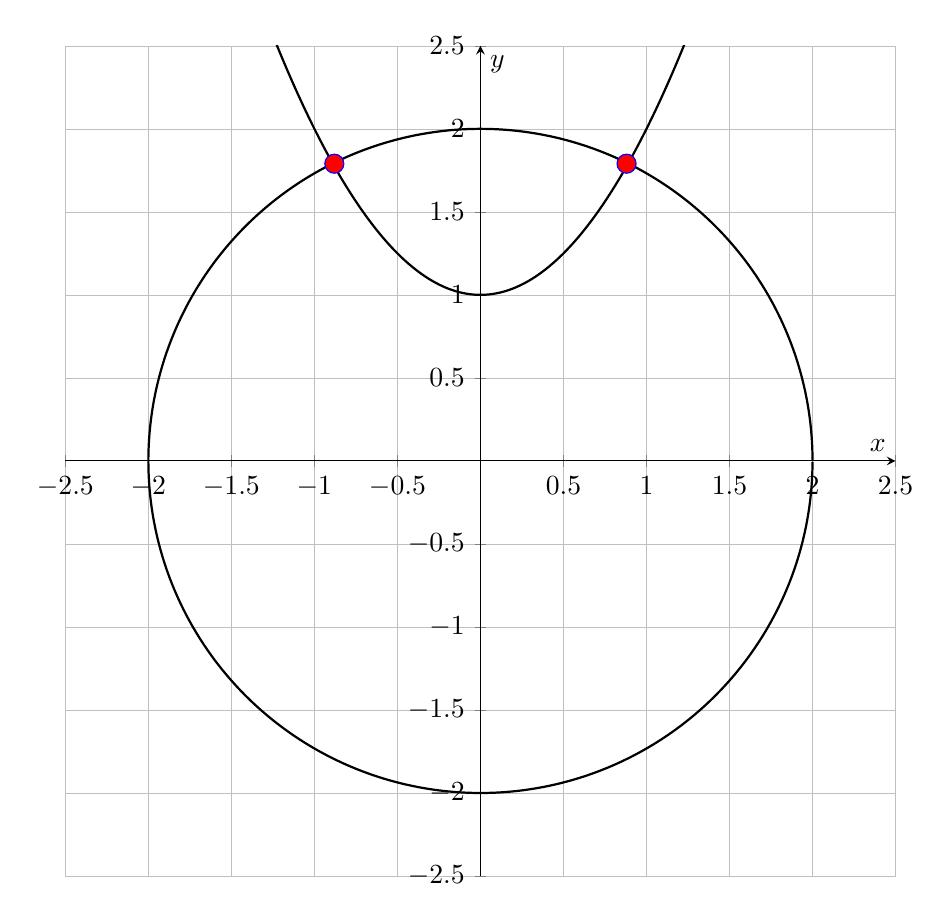
\begin{tikzpicture}
    \begin{axis}[
      axis lines=middle,
      xmin=-2.5,xmax=2.5,
      ymin=-2.5,ymax=2.5,
      xlabel={\(x\)},
      ylabel={\(y\)},
      grid=both,
      grid style={line width=.1pt, draw=gray!20},
      major grid style={line width=.2pt,draw=gray!50},
      width=\textwidth, height=\textwidth
    ]
    
    \coordinate (r0) at (0.88,1.79);
    \coordinate (r1) at (-0.88,1.79);
    
    
    % Draw the circle x^2 + y^2 = 4
    \addplot [samples=200, domain=0:2*3.14, smooth, thick] ({2*cos(deg(x))}, {2*sin(deg(x))});
    
    % Draw the parabola y = x^2 + 1
    \addplot [samples=200, domain=-2:2, smooth, thick] {x^2 + 1};
    
    \draw[fill=red, draw=blue] (r0) circle (0.01\textwidth);
    \draw[fill=red, draw=blue] (r1) circle (0.01\textwidth);
    
    \end{axis}
    \end{tikzpicture}
    \end{columns}
  \end{frame}
  
  \begin{frame}[fragile]
    \frametitle{Newton-Raphson Method: multi-dimensional case}
  
    \textbf{Extensions to multi-dimensional case:}
  
    \textbf{Check order of convergence:}
  
    \[
    \begin{array}{|c|c|c|c|c|c|c|}
    \hline
    \text{it} & x_1 & x_2 & \text{eps1} & \text{eps2} & m_1 & m_2 \\
    \hline
    1 & 1.0000 & 2.0000 & & & & \\
    2 & 0.9000 & 1.8000 & 0.1000 & 0.2000 & & \\
    3 & 0.8896 & 1.7913 & 0.0104 & 0.0087 & 1.9835 & 2.9482 \\
    4 & 0.8895 & 1.7913 & 0.0000699 & 0.0000165 & 2.0949 & 2.3208 \\
    5 & 0.8895 & 1.7913 & 0.0000000278 & 0.0000000059 & 2.0589 & 2.1382 \\
    \hline
    \end{array}
    \]
    
    \begin{block}{Quadratic convergence}
    Doubling number of significant digits every iteration
    \end{block}
    \[
    m = \frac{\ln(\varepsilon_{n+1}) - \ln(\varepsilon_n)}{\ln(\varepsilon_n) - \ln(\varepsilon_{n-1})}
    \]
  \end{frame}

  \begin{frame}[fragile]
    \frametitle{Newton-Raphson Method}
    
    \textbf{Deriving the extension to more than two variables}:
    \begin{columns}
      \begin{column}{0.5\textwidth}
        \begin{enumerate}
          \item Generalization to the N-dimensional case
          \item Define variables
          \item Multi-variate Taylor series expansion
          \item Define Jacobian matrix
          \item Neglect higher-order terms
          \item Express in terms of iterations
        \end{enumerate}
      \end{column}
      \begin{column}{0.5\textwidth}
        \begin{enumerate}
          \item 
            \( f_i(x_1, x_2, \ldots, x_N) = 0 \)
          \item 
            \( \mathbf{x} = [x_1, x_2, \ldots, x_N] \)
            \( \mathbf{f} = [f_1, f_2, \ldots, f_N] \)
          \item 
            \( f_i(\mathbf{x} + \delta \mathbf{x}) = f_i(\mathbf{x}) + \sum_{j=1}^{N} \frac{\partial f_i}{\partial x_j} \delta x_j + O(\delta \mathbf{x}^2) \)
          \item 
            \( J_{ij} = \frac{\partial f_i}{\partial x_j} \)
            \( f(\mathbf{x} + \delta \mathbf{x}) = f(\mathbf{x}) + \mathbf{J} \delta \mathbf{x} + O(\delta \mathbf{x}^2) \)
          \item 
            \( \mathbf{J} \cdot \delta \mathbf{x} = -\mathbf{f}(\mathbf{x}) \)
        \end{enumerate}
      \end{column}
    \end{columns}
    \[
      \boxed{\mathbf{x}_{n+1} = \mathbf{x}_n-\mathbf{J}^{-1}(\mathbf{x}_n)\cdot\mathbf{f}(\mathbf{x}_n)}
    \]
  \end{frame}
  
  
  \begin{frame}[fragile]
    \frametitle{Newton-Raphson Method}
    
    Multi-variate Newton-Raphson in Python:
    \begin{columns}
      \column{0.5\textwidth}
      \begin{lstlisting}[language=Python, basicstyle=\tiny]
def my_equations(X):
    F = np.zeros(2)
    F[0] = X[0]**2 + X[1]**2 - 4
    F[1] = X[0]**2 - X[1] + 1
    return F
      \end{lstlisting}
      \column{0.5\textwidth}
      \begin{lstlisting}[language=Python, basicstyle=\tiny]
def my_jac(x):
    jac = np.zeros((2, 2))
    jac[0, 0] = 2 * x[0]
    jac[0, 1] = 2 * x[1]
    jac[1, 0] = 2 * x[0]
    jac[1, 1] = -1
    return jac
      \end{lstlisting}
    \end{columns}
    \begin{lstlisting}[language=Python, basicstyle=\tiny]
import numpy as np
def newton_nd(f, J, x0, tol, max_iter):
    x = np.array(x0)
    err = np.zeros(max_iter)
    p = np.zeros(max_iter)
    for i in range(max_iter):
        delta_x = -np.linalg.solve(J(x), f(x))
        x += delta_x
        err[i] = np.linalg.norm(delta_x)
        if i > 0:
            p[i] = np.log(err[i]) / np.log(err[i-1])
        else:
            p[i] = float('nan')
        print(f'i = {i}: x = {x}, err = {err[i]:.6e}, p = {p[i]:.6f}')
        if err[i] < tol:
            break
    return x
    \end{lstlisting}
    \begin{lstlisting}[language=Python]
newton_nd(my_equations, my_jac, [1, 2], 1e-12, 100)
    \end{lstlisting}
\end{frame}


  \begin{frame}[fragile]
    \frametitle{Newton-Raphson Method}
  
    \textbf{Multi-variate Newton-Raphson in Python:}
    
    Plotting the functions:
    \begin{lstlisting}[language=Python]
plot_implicit_function(lambda x,y: y-x**2, resolution=100, colors="blue")
plot_implicit_function(lambda x,y: y**2+x**2-4, resolution=100, colors="red")
    \end{lstlisting}
    \begin{columns}
      \column{0.5\textwidth}
      \includegraphics[width=\textwidth]{circle_and_parabola_python.pdf}
      \column{0.5\textwidth}
      \begin{itemize}
        \item Code can be found in \lstinline[language=Python]{plot_implicit.py}
        \item Uses contour plot at $f(x,y)=0$
      \end{itemize}
      % \lstinputlisting[language=Python, basicstyle=\tiny]{scripts/plot_implicit.py}
    \end{columns}
  \end{frame}

  
\begin{frame}[fragile]
  \frametitle{Newton-Raphson Method}

  \textbf{Multi-variate Newton-Raphson in Python:}
  
  Plotting the norm of the function:
  \begin{lstlisting}[language=Python]
plot_surface_function(lambda x,y: np.sqrt((x**2 + y**2 -4)**2+(x**2-y+1)**2),
                         (0,3),(0,3))
        \end{lstlisting}
        \begin{columns}
          \column{0.5\textwidth}
          \includegraphics[width=0.8\textwidth]{surface_circ_par_error.pdf}
          \column{0.5\textwidth}
          \begin{itemize}
            \item Code can be found in \lstinline[language=Python]{plot_implicit.py}
            \item Uses contour plot at $f(x,y)=0$
          \end{itemize}
          % \lstinputlisting[language=Python, basicstyle=\tiny]{scripts/plot_implicit.py}
        \end{columns}
\end{frame}

\begin{frame}[fragile]
  \frametitle{Newton-Raphson Method}

  \textbf{Multi-variate Newton-Raphson in Python:}
  
  Plotting the norm of the function:
  \begin{lstlisting}[language=Python]
plot_contours(lambda x,y: np.sqrt((x**2 + y**2 -4)**2+(x**2-y+1)**2),
                 (0, 3), (0, 3), resolution = 100, levels=[0, 1, 2, 3, 4])
        \end{lstlisting}
        \begin{columns}
          \column{0.5\textwidth}
          \includegraphics[width=0.8\textwidth]{surface_circ_par_error_contour.pdf}
          \column{0.5\textwidth}
          \begin{itemize}
            \item Code can be found in \lstinline[language=Python]{plot_implicit.py}
            \item Uses contour plot at $f(x,y)=0$
          \end{itemize}
          % \lstinputlisting[language=Python, basicstyle=\tiny]{scripts/plot_implicit.py}
        \end{columns}
\end{frame}

  \begin{frame}[fragile]
    \frametitle{Broyden's Method}
    
    \textbf{Multi-dimensional secant method ('quasi-Newton'):}
    \begin{itemize}
      \item Disadvantage of the Newton-Raphson method:
        \begin{itemize}
          \item It requires the Jacobian matrix.
          \item In many problems, no analytical Jacobian is available.
          \item If the function evaluation is expensive, the numerical approximation using finite differences can be prohibitive.
        \end{itemize}
      \item Solution: Use a cheap approximation of the Jacobian! (Secant or 'quasi-Newton' method)
      \item Comparison:
        \[
        \text{Newton-Raphson:} \quad J_{ij}(\mathbf{x}) = \frac{\partial f_i}{\partial x_j}(\mathbf{x}) \quad \text{(Analytical)}
        \]
        \[
        \text{Secant method:} \quad \mathbf{J}(\mathbf{x}) \quad \text{approximated by}\quad \mathbf{B} \quad \text{(Numerical)}
        \]
    \end{itemize}
  \end{frame}

  \begin{frame}[fragile]
    \frametitle{Broyden's Method}
  
    \textbf{Approximating $\mathbf{B}^{n+1}$:}
    \begin{itemize}
      \item Multi-dimensional secant method ('quasi-Newton'):
      \item Secant equation (generalization of 1D case):
      \[
        \mathbf{B}^{n+1} \cdot \delta \mathbf{x}^n=\delta \mathbf{f}^n \quad \delta \mathbf{x}^n=\mathbf{x}^{n+1}-\mathbf{x}^n \quad \delta \mathbf{f}^n=\mathbf{f}^{n+1}-\mathbf{f}^n
      \]
      \item Underdetermined (not unique: -n equations with n unknowns), need another condition to pin down \(B^{n+1}\).
    \end{itemize}
    \textbf{Broyden's method:}
    \begin{itemize}
      \item  Determine \(\mathbf{B}^{n+1}\) by making the least change to \(\mathbf{B}^{n}\) that is consistent with the secant condition.
      \item Updating formula:
      \[
        \mathbf{B}^{n+1}=\mathbf{B}^n+\frac{\left(\delta \mathbf{f}^n-\mathbf{B}^n \cdot \delta \mathbf{x}^n\right)}{\delta \mathbf{x}^n \cdot \delta \mathbf{x}^n} \otimes \delta \mathbf{x}^n
      \]
      \item Note: Sometimes \(\delta B_{n-1}\) is updated directly.
    \end{itemize}
  \end{frame}
  
  \begin{frame}[fragile]
    \frametitle{Broyden's Method}
  
    \textbf{Background of Broyden’s method:}
    \begin{itemize}
      \item Secant equation:
      \[
      \textbf{B}^{n+1} \cdot \delta \textbf{x}^n = \delta f_{n}
      \]
      \item Since there is no update on derivative info, why would \(\textbf{B}^{n}\) change in a direction orthogonal to \(\delta \textbf{x}^n\)?
      \[
        \Rightarrow (\delta \textbf{x}^n)^T \delta \textbf{w} = 0
      \]
      % \item Updating formula:
      \vspace{-0.5cm}
      \begin{columns}
        \column{0.1\textwidth}
        \column{0.2\textwidth}
        \begin{align*}
          &\textbf{B}^{n+1}\cdot\textbf{w} = \textbf{B}^{n}\cdot\textbf{w}\\
          &\textbf{B}^{n+1}\cdot\delta \textbf{x}^n = \delta \textbf{f}^n
        \end{align*}
        \column{0.05\textwidth}
        \[
          \Rightarrow  
        \]
        \column{0.65\textwidth}
        \[
          \mathbf{B}^{n+1}=\mathbf{B}^n+\frac{\left(\delta \mathbf{f}^n-\mathbf{B}^n \cdot \delta \mathbf{x}^n\right)}{\delta \mathbf{x}^n \cdot \delta \mathbf{x}^n} \otimes \delta \mathbf{x}^n
        \]
      \end{columns}
      \vspace{0.5cm}
      \item Initialize \(\delta \textbf{x}^n\) and \(\textbf{B}_{0}\) with the identity matrix (or with finite difference approx.).
    \end{itemize}
  \end{frame}


  \begin{frame}[fragile]
    \frametitle{Broyden's Method}
    \textbf{Python implementation of Broyden's method:}
    \begin{columns}
      \column{0.5\textwidth}
    \begin{itemize}
      \item Same example as before but now with Broyden's method.
      \item Slower convergence with Broyden's method should be offset by improved efficiency of each iteration!
      \begin{lstlisting}[language=Python]
broyden(@MyFunc,[1;2],1e-12,1e-12)
      \end{lstlisting}
      \item Requires 11 iterations (compare with Newton: 5 iterations)
      
      But much fewer function evaluations per iteration!
    \end{itemize}
  
    \column{0.5\textwidth}
    \begin{lstlisting}[language=Python]
import numpy as np
from numpy.linalg import inv

def broyden(F, x0, tol=1e-6, max_iter=100):
    x = np.array(x0)
    B = np.eye(x.size)
    for i in range(max_iter):
        Fx = F(x)
        if np.linalg.norm(Fx) < tol:
            print(f"Converged after {i} iterations.")
            return x
        x_new = x - inv(B)@Fx
        delta_x = x_new - x
        delta_Fx = F(x_new) - Fx
        B += np.outer((delta_Fx - B@delta_x)/(delta_x@delta_x), delta_x)
        x = x_new
    print("Max iterations reached.")
    return x
    \end{lstlisting}
  \end{columns}
  \end{frame}

  
  \begin{frame}[fragile]
    \frametitle{Broyden's Method}
  
    \begin{itemize}
      \item Same example as before but now with Broyden's method.
      \item Note how the approximate Jacobian (\(\textbf{B}\)) is updated over subsequent iterations:
      
      \begin{tiny}
        \begin{align*}
          \begin{bmatrix}
          1. & 0. \\
          0. & 1.
          \end{bmatrix} & \rightarrow &
          \begin{bmatrix}
          3. & -1. \\
          4. & -1.
          \end{bmatrix} & \rightarrow &
          \begin{bmatrix}
          -1.0 & -9.0 \\
          3.4 & -2.2
          \end{bmatrix} & \rightarrow &
          \begin{bmatrix}
          -1.062 & -9.260 \\
          3.411 & -2.154
          \end{bmatrix} & \rightarrow &\\
          \begin{bmatrix}
          5.290 & -3.864 \\
          2.493 & -2.934
          \end{bmatrix} & \rightarrow &
          \begin{bmatrix}
          7.363 & -1.931 \\
          3.556 & -1.943
          \end{bmatrix} & \rightarrow &
          \begin{bmatrix}
          2.349 & -0.773 \\
          3.547 & -1.941
          \end{bmatrix} & \rightarrow &
          \begin{bmatrix}
          -0.934 & -6.772 \\
          2.351 & -4.124
          \end{bmatrix} & \rightarrow &\\
          \begin{bmatrix}
          -0.384 & -5.879 \\
          2.500 & -3.884
          \end{bmatrix} & \rightarrow &
          \begin{bmatrix}
          10.416 & 6.344 \\
          5.947 & 0.018
          \end{bmatrix} & \rightarrow &
          \begin{bmatrix}
          9.781 & 5.515 \\
          5.641 & -0.382
          \end{bmatrix} & \rightarrow &
          \begin{bmatrix}
          3.577 & 3.630 \\
          3.362 & -1.074
          \end{bmatrix} & \rightarrow &\\
          \begin{bmatrix}
          3.116 & 3.238 \\
          2.912 & -1.458
          \end{bmatrix} & \rightarrow &
          \begin{bmatrix}
          1.992 & 3.272 \\
          1.989 & -1.430
          \end{bmatrix} & \rightarrow & \hdots & \rightarrow & \hdots & \rightarrow &
  \end{align*}  
    \end{tiny}

    \item Compare with analytical jacobian:
    \(
      \textbf{B}=\begin{bmatrix}
      1.748 & 3.261 \\
      1.736 & -1.439
      \end{bmatrix}\quad
      \textbf{J}=
      \begin{bmatrix}
      1.779 & 3.583 \\
      1.779 & -1
      \end{bmatrix}
      \)
      \item Note that the approximate Jacobian (\(\textbf{B}\)) is not exact even when the solution has already been found!
    \end{itemize}
  \end{frame}
  
  \begin{frame}[fragile]
    \frametitle{Conclusions}
  
    \begin{itemize}
      \item Recommendations for root finding:
      \begin{itemize}
        \item One-dimensional cases:
        \begin{itemize}
          \item If it is not easy/cheap to compute the function's derivative $\Rightarrow$ use Brent's algorithm.
          \item If derivative information is available $\Rightarrow$ use Newton-Raphson's method + bookkeeping on bounds provided you can supply a good enough initial guess!!
          \item There are specialized routines for (multiple) root finding of polynomials (but not covered in this course).
        \end{itemize}
        \item Multi-dimensional cases:
        \begin{itemize}
          \item Use Newton-Raphson method, but make sure that you provide an initial guess close enough to achieve convergence.
          \item In case derivative information is expensive $\Rightarrow$ use Broyden's method (but slower convergence!).
        \end{itemize}
      \end{itemize}
    \end{itemize}
  \end{frame}
  
  